% Copyright (C) 2005-2015 Airbus - EDF - IMACS - Phimeca
% Permission is granted to copy, distribute and/or modify this document
% under the terms of the GNU Free Documentation License, Version 1.2
% or any later version published by the Free Software Foundation;
% with no Invariant Sections, no Front-Cover Texts, and no Back-Cover
% Texts.  A copy of the license is included in the section entitled "GNU
% Free Documentation License".

\documentclass[a4paper,11pt]{article}

\usepackage[utf8]{inputenc}
\usepackage{graphicx}
\usepackage{listings}
\lstset{basicstyle=\color{blue}}
\usepackage{fancyhdr}
\usepackage{color}
\usepackage{float}
\usepackage{makeidx}

\usepackage{otcommon}

\pagestyle{fancy}
\fancyhf{} \rhead{\bfseries \thepage} \lhead{\bfseries \nouppercase OpenTURNS -- Developer's guide}
\rfoot{\bfseries \copyright 2005-2015 Airbus - EDF - IMACS - Phimeca} \lfoot{}

% For OpenTURNS standard math notations
\usepackage{Math_Notations}

% fonts for the table and figure captions
\usepackage[small,bf,up]{caption}
%\newcommand{\captionfont}{\small\itshape}

% macros used in the document
\newcommand{\OT} {OpenTURNS}
\newcommand{\Sal} {Salom\'e}

\makeindex

\begin{document}

\begin{titlepage}
  \vspace*{2cm}
  \begin{center}
    {\huge \bf Developer's guide}
    \input{GenericInformation.tex}
  \end{center}

\end{titlepage}

\newpage

% \input{summary}

\cleardoublepage
% depth of the TOC
% \setcounter{tocdepth}{4}
\tableofcontents
\cleardoublepage
\listoffigures
\cleardoublepage
\listoftables
\cleardoublepage

\section*{Introduction}

This document introduces \OT\ from the developer's point of view.

\subsection*{Document outline}
The document is organized as follows:
\begin{itemize}
\item \emph{Chapter 1} makes up the general specifications for the architecture of the \OT\ platform;
\item \emph{Chapter 2} aims at presenting some elements to ease the work of contributors;
\item \emph{Chapter 3} describes how to develop a module;
\item \emph{Chapter 4} shows how to create wrappers around external codes.
\end{itemize}

\cleardoublepage

\section{Architecture}
% Copyright (C) 2005-2015 Airbus - EDF - IMACS - Phimeca.
% Permission is granted to copy, distribute and/or modify this document
% under the terms of the GNU Free Documentation License, Version 1.2
% or any later version published by the Free Software Foundation;
% with no Invariant Sections, no Front-Cover Texts, and no Back-Cover
% Texts.  A copy of the license is included in the section entitled "GNU
% Free Documentation License".

The \OT\ project is an open source project. It aims at developing a computational platform designed to carry out industrial studies on uncertainty processing and risk analysis.

This platform is intended to be released as an open source contribution to a wide audience whose technical skills are very diverse. Another goal of the project is to make the community of users ultimately responsible for the platform and its evolution by contributing to its maintenance and developing new functions.

This architecture specifications document therefore serves two purposes:
\begin{itemize}
\item to provide the design principles that govern the platform, in order to guide the development teams in their development process;
\item to inform external users about the platform's architecture and its design, in order to facilitate their first steps with the platform.
\end{itemize}

% In the first section of this document, we will introduce the concepts that governed the construction of the platform. These concepts resulted from the requirements analysis carried out with the users and the developers, following the UML approach. The general functions of the platform allowed us to categorize the concepts by giving us a more synthetic and global view of its components.
%
%
% The second section details the technical choices that were retained for the platform's development.

To address these questions, the \OT\ platform needs to be:
\begin{itemize}
\item \emph{portable}: the ability to build, execute and validate the application in different environments (operating system, hardware platform as well as software environment) based on a single set of source code files.
\item \emph{extensible}: the possibility to add new functions to the application with a minimal impact on the existing code.
\item \emph{upgradable}: the ability to control the impact of a replacement or a change on the technical architecture, following an upgrade of the technical infrastructure (such as the replacement of one tool by another or the use of a new storage format).
\item \emph{durable}: the technical choices must have a lifespan comparable to the application's while relying on standard and/or open source solutions.
\end{itemize}


\subsection{Overview}

This chapter will describe the general design of \OT\, and a few design models that are widely used within the platform.

The core of OpenTURNS platform is a C++ library made of about 500 classes of various size.

The main user interface is a python module, automatically generated from the C++ library using the wrapping software SWIG. It allows for a usage of OpenTURNS through python scripts of any level of complexity.

The library relies on relatively few dependencies, (Lapack, R, TBB, LibXml2), and most of them are optional.

Several GUIs have already been built on top of the C++ library or the Python module.

A service of modules is provided in order to extend the capabilities of the platform from the outside.

\begin{figure}[H]
\begin{center}
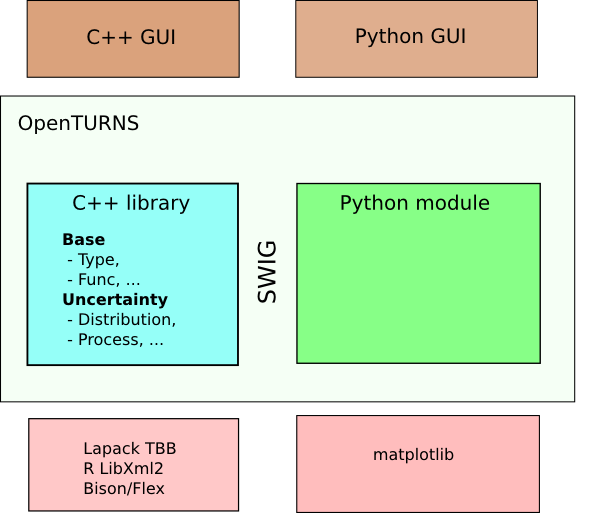
\includegraphics[scale=0.5]{Figures/architecture.png}
\caption{Software architecture overview}
\end{center}
\end{figure}

\subsubsection{The C++ library}

\paragraph{A multi-layered library}

The library has a multi-layered architecture materialized by the source tree.
The two main layers in the C++ library are the Base layer and the Uncertainty layer.
\begin{itemize}
\item Base layer: it contains all the classes not related to the probabilistic concepts. It covers the elementary data types (vectors as NumericalPoint, samples as NumericalSamples), the concept of models (NumericalMathFunction), the linear algebra (Matrix, Tensor) and the general interest classes (memory management, resource management);
\item Uncertainty layer: it contains all the classes that deal with probabilistic concepts. It covers the probabilistic modelling (Distribution, RandomVector), the stochastic algorithms (MonteCarlo, FORM), the statistical estimation (DistributionFactory), the statistical testing (FittingTest)
\end{itemize}
A class in the Uncertainty layer can use any class in the Base or the Uncertainty layer. A class in the Base layer can ONLY USE classes in the Base layer.

\paragraph{Resource management}

OpenTURNS uses extensively dynamic memory allocation. In order to tie to the Resource Acquisition Is Initialization (RAII) paradigm, all the memory management is delegated to smart pointers (the Pointer class). The benefits of this approach are:
\begin{itemize}
\item An easy to implement copy on write mechanism, that permit a significant reduction of the memory footprint by allowing for a large data sharing between objects;
\item No C-like pointers in members of classes, which permits an automatic generation of the copy constructor, the assignment operator and the destructor of almost all the classes: there is no problem of deep copy versus reference copy;
\item The resource is released automatically when the objects are outside of the current scope and there is no more reference on the allocated memory;
\item There is a unique point where to prevent concurrent access in a parallel context, which is a key property for parallelism.
\end{itemize}

\subsubsection{The Python module}

The binding of the library is done almost automatically by SWIG (Simplified Wrapper Interface Generator) through a set of SWIG interface files (.i).\\
The main target language is python.
These swig files contain some specific 'glue code' to each class for the target script language.
SWIG parses the library headers and theses swig interface files to generates the corresponding module source yet to be compiled to produce a binary python module, see \ref{fig:swig}.
The process is shared between several modules for modularity and to speed up compilation time with parallel builds.

\begin{figure}[H]
\begin{center}
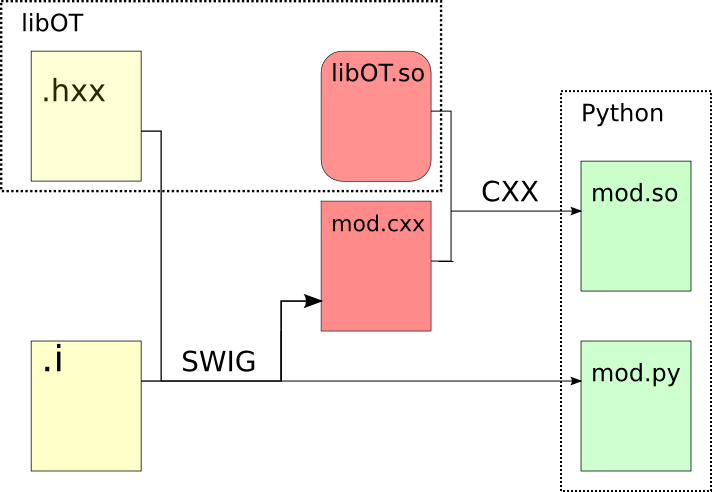
\includegraphics[scale=0.5]{Figures/design/swig.png}
\caption{Python module generation process}\label{fig:swig}
\end{center}
\end{figure}

\subsection{Software environment}

This section details the technical elements required by the OpenTURNS platform, namely the system requirements, the tools and the development environment of the project.

\subsubsection{Target platforms}

The OpenTURNS platform is meant to carry out uncertainty treatment studies in a scientific environment. Most of the scientific codes being available on Unix platforms, OpenTURNS is naturally designed to run on this family of systems. Unix being a standard with multiple implementations, available on different architectures, this gives a wide choice of target platforms.

Linux is currently the most attractive Unix system for the OpenTURNS project, it was chosen as the main target system for the project's development as well as for the delivery of the different versions.

The partners involved in the project have each chosen different Linux distributions, for technical and historical reasons. Therefore, it was decided to support several distributions, a choice that should not be seen as final or minimal. The distributions considered here include for example the list given in Table \ref{linux}

\begin{center}
\begin{table}[h]
\caption{\label{linux}Operating systems supported by the project's partners}
\begin{center}
\begin{tabular}{|l|l|}
\hline
\textbf{Distribution} & \textbf{Version} \\
\hline \hline
Debian & 6 "Squeeze" \\
Ubuntu & 12.04 "Precise" \\
Windows & XP \\
Windows & 7 \\
\hline
\end{tabular}
\end{center}
\end{table}
\end{center}

The primary development platform is Linux, and is known to work on various other distributions.

The Windows version is obtained by cross-compilation using MinGW.

\subsubsection{Dependencies}

The tools chosen for the development of the platform are listed in Table \ref{tools}

\begin{center}
\begin{table}[h]
\caption{\label{tools}Software development tools}
\begin{center}
\begin{tabular}{|l|l|l|}
\hline
\textbf{Category} & \textbf{Name} & \textbf{Version} \\
\hline \hline
Configuration & CMake & 2.8 or later \\
C/C++/Fortran compiler & Gcc & 3.3.5 or later \\
Linear algebra & BLAS & 3.0 or later \\
Linear algebra & LAPACK & 3.0 or later \\
Analytical parser (optional) & muParser & 1.32 or later \\
Distribution functions (optional) & Boost & 1.46 or later \\
CSV parser (optional) & flex & 2.5.33 or later \\
CSV parser (optional) & bison & 2.4 or later \\
XML support (optional) & LibXml2 & 2.6.27 \\
Multithreading (optional) & TBB & 2 or later \\
Python support & Python & 2.3.5 or later \\
Plotting library (optional) & matplotlib & 1.1 or later \\
C++/Python wrapper & SWIG & 1.3.35 or later \\
Statistics library (optional) & R & 2.0.1 or later \\
Calculator (optional for some test) & bc & 1.06 or later \\
Version control & Subversion & 1.1 or later \\
LaTeX to XML (optional for doc) & Tralics & 2.14.5 or later \\
\hline
\end{tabular}
\end{center}
\end{table}
\end{center}

The versions given here are only meant as indications and other versions may be used. However, in case of compatibility issues arising from the use of other packages than those suggested here, support may not be the responsibility of the project.

\subsubsection{Compilation infrastructure}

The historic autotools compilation infrastructure was replaced by CMake. CMake is a lot faster, and the resulting infrastructure is easier to maintain. It covers:
\begin{itemize}
\item The detection and configuration aspects of the platform;
\item The dependency management of the sources;
\item The generation of parallel makefiles;
\item The regression tests.
\end{itemize}
CMake could also provide a way to compile the Windows version using Microsoft compilers.

\subsubsection{Packaging}

The \OT\ team officially provides binaries for the Debian operating system, and Windows.
Note that \OT\ is officially supported in Debian: it can be installed easily from the debian software repositories.
Experimental packages may be available for some RPM-based distributions such as Fedora, CentOS and OpenSUSE.

\subsubsection{Autobuilder}

\OT\ provides developers with a continuous integration environment.
It consists in an daemon monitoring the version control software for changes.
It assumes new code to be involved in regression test.
Also developers should regularly commit to the code base to ensure the origin of a problem is quickly detected.

The autobuilder is triggered by the keyword '\verb|distcheck ok|' in the commit log.

The current test environment consists of the build on each of these platforms:
\begin{itemize}
\item debian 6 x86\_64
\item debian 6 i686
\item windows i686 (wine)
\end{itemize}
The result of the autobuilder made public to anyone registered to the mailing list \verb|commits@openturns.org|.
A summary of each build is provided by mail with links to the logs stored on the server.

\subsection{Design patterns}

\subsubsection{Introduction}

Software design shows the recurrence of some patterns, whether within the same piece of software or in several applications (which can differ in many ways). These patterns have been catalogued, described and implemented in numerous situations that prove their universality and their ability to solve recurring problems that the software architect is faced with.

The following sections give an overview intended as much for the reader's understanding of the document as to establish a common vocabulary for software architect. The latter ones will find here standard design diagrams applied to the specific case of \OT, which can help them better apprehend the tool's specificities and the design and implementation choices that were made.

\label{bridge}\subsubsection{Bridge pattern}

The bridge pattern is a design pattern used in software engineering which is meant to "decouple an abstraction from its implementation so that the two can vary independently". The bridge uses encapsulation, aggregation, and can use inheritance to separate responsibilities into different classes.\\
When a class varies often, the features of object-oriented programming become very useful because changes to a program's code can be made easily with minimal prior knowledge about the program. The bridge pattern is useful when both the class as well as what it does vary often. The class itself can be thought of as the implementation and what the class can do as the abstraction. The bridge pattern can also be thought of as two layers of abstraction.

This pattern is one of the most widely used in \OT. Some examples are:
\begin{itemize}
\item Drawable, that separate the generic high level interface of a drawable from the specific low level interface of the several drawable specializations;
\item Distribution, see \ref{fig:bridge}, that exposes a high level interface of the concept of probability distribution whereas the DistributionImplementation class exposes the low level interface of the same concept.
\end{itemize}

\begin{figure}[htb]
\begin{center}
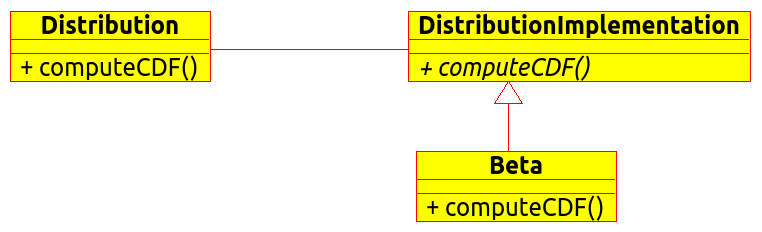
\includegraphics[scale=0.5]{Figures/modeling_notions/bridge.png}
\caption{Bridge pattern example.}\label{fig:bridge}
\end{center}
\end{figure}


\label{singleton}\subsubsection{Singleton pattern}

The Singleton is a pattern used to ensure that at any given time, there is only one instance of a class (A); it provides an access point for this unique instance.

This is implemented by creating a class (Singleton) with a static private attribute (uniqueInstance) initialized with an instance of class A and whose reference (or pointer) is returned by a static method (instance). Figure \ref{fig:singleton} illustrates the Singleton pattern.

\begin{figure}[htb]
\begin{center}
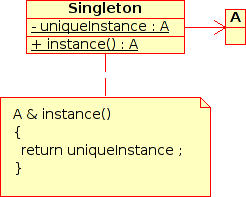
\includegraphics[scale=0.5]{Figures/modeling_notions/singleton.png}
\caption{Singleton structure.}\label{fig:singleton}
\end{center}
\end{figure}

It is a very common pattern that allows to find and share an object (which must remain unique) in different portions of code.
Examples of such objects include shared hardware resources (standard output, error, log, etc.), but also internal functions that cannot or must not be duplicated (e.g. a random number generator).
For example, the classes ResourceMap and IdFactory follow this pattern.

\label{factory}\subsubsection{Factory pattern}

This pattern allows to define a unique interface for the creation of objects belonging to a class hierarchy without knowing in advance their exact type.
Figure \ref{fig:factory} illustrates this pattern.
The creation of the concrete object (ClassA or ClassB) is delegated to a sub-class (ClassAFactory or ClassBFactory) which chooses the type of object to be created and the strategy to be used to create it.

\begin{figure}[htb]
\begin{center}
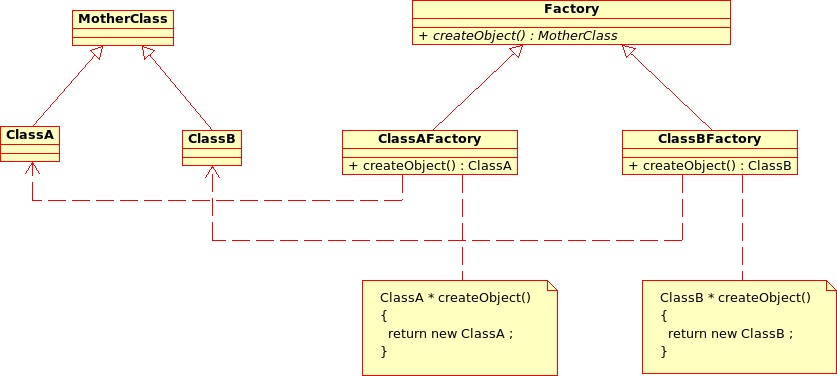
\includegraphics[scale=0.5]{Figures/modeling_notions/factory.png}
\caption{Factory structure.}\label{fig:factory}
\end{center}
\end{figure}

This pattern is often used to dynamically create objects belonging to related types (e.g. to instantiate objects within a GUI according to the user's behavior).
It can also be used to back up and read again a document written in a file by automatically re-instantiating objects.
It is a pattern that makes code maintenance easier by clearly separating the objects and their instantiation in distinct and parallel class hierarchies.
For example, the classes DistributionFactory, ApproximationAlgorithmImplementationFactory, BasisSequenceFactory follow this pattern.

\label{strategy}\subsubsection{Strategy pattern}

The Strategy pattern defines a family of algorithm and makes them interchangeable as far as the client is concerned. Access to these algorithms is provided by a unique interface which encapsulates the algorithms' implementation. Therefore, the implementation can change without the client being aware of it.

\begin{figure}[htb]
\begin{center}
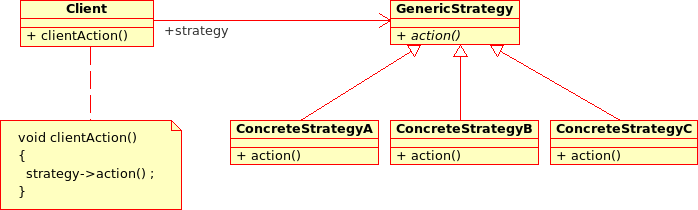
\includegraphics[scale=0.5]{Figures/modeling_notions/strategy.png}
\caption{Strategy structure.}\label{fig:strategy}
\end{center}
\end{figure}

This pattern is very useful to provide a client with different implementations of an algorithm which are equivalent from a functional point of view. It can be noted that the Factory pattern described earlier makes use of the Strategy pattern.
For example, the classes ComparisonOperator, HistoryStrategy follow this pattern.

\label{composite}\subsubsection{Composite pattern}

The Composite pattern is used to organize objects into a tree structure that represents the hierarchies between component and composite objects. It hides the complex structure of the object from the client handling the object.

\begin{figure}[htb]
\begin{center}
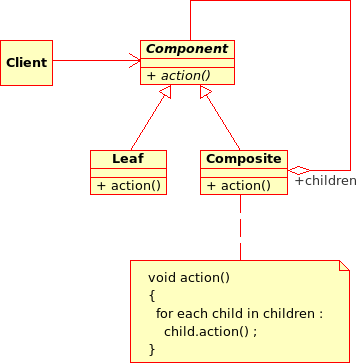
\includegraphics[scale=0.5]{Figures/modeling_notions/composite.png}
\caption{Composite structure.}\label{fig:composite}
\end{center}
\end{figure}

Figure \ref{fig:composite_tree} shows an example of tree modeled by the Composite. The Composite objects make up the tree nodes whereas the leaves can be any concrete object deriving from Component.

\begin{figure}[htb]
\begin{center}
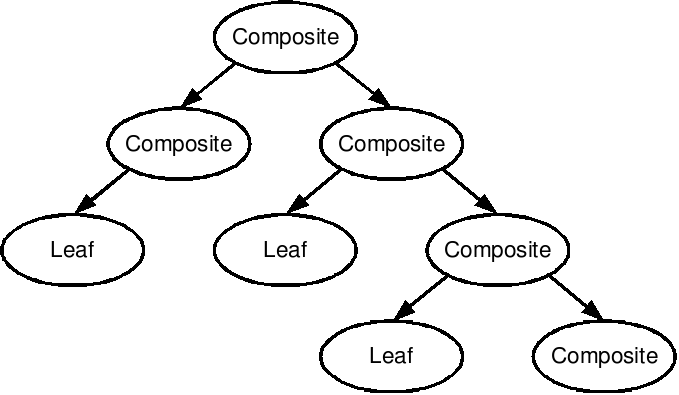
\includegraphics[scale=0.45]{Figures/modeling_notions/composite_tree.png}
\caption{Example of tree modeled by the Composite.}\label{fig:composite_tree}
\end{center}
\end{figure}

The Composite pattern is an essential element of the design model for the \OT\ platform. It can be used to model numerical function composition, random vector composition, etc. It can be found in several aspects of the modeling brick. Any related objects tree structure can rely on the Composite pattern with benefit.
For example, the classes ComposedDistribution, CompositeRandomVector, ComposedNumericalMathFunction follow this pattern.

\cleardoublepage

\section{Platform development}
% Copyright 2005-2016 Airbus-EDF-IMACS-Phimeca
% Permission is granted to copy, distribute and/or modify this document
% under the terms of the GNU Free Documentation License, Version 1.2
% or any later version published by the Free Software Foundation;
% with no Invariant Sections, no Front-Cover Texts, and no Back-Cover
% Texts.  A copy of the license is included in the section entitled "GNU
% Free Documentation License".

This section provides informations on how to develop within the perimeter of the library and it's documentation.

\newcounter{oldenumi}

\subsection{Install a development version of OpenTURNS}

\subsubsection{Install the required dependencies}

See \ref{tools}, for the system requirements.

\subsubsection{Download openturns}

You can retrieve the development master branch through the scm repository by issuing the following command:
\begin{lstlisting}
svn co https://svn.openturns.org/openturns/trunk
cd trunk
\end{lstlisting}

Or, you can pick up a stable version tarball:
\begin{lstlisting}
wget http://downloads.sourceforge.net/openturns/openturns/openturns-1.1.tar.bz2
tar xjf openturns-1.1.tar.bz2
cd openturns-1.1
\end{lstlisting}

You may want to install the provided R package enabling additional statistical capabilities:
\begin{lstlisting}
R CMD INSTALL utils/rot_1.4.5.tar.gz
\end{lstlisting}

You can verify it's correct installation by typing:
\begin{lstlisting}
R --vanilla <<< 'library(rot)'
\end{lstlisting}

\subsubsection{Build openturns}

\begin{lstlisting}
mkdir build
cd build
cmake -DCMAKE_INSTALL_PREFIX=$PWD/install ..
make install -j4
\end{lstlisting}

\subsubsection{Run tests}
\begin{lstlisting}
make tests
ctest -j4
\end{lstlisting}
and all the tests should be successful else check the log file Testing/Temporary/LastTest.log.

\subsection{Adding a class to an existing directory \label{SingleClass}}

This how-to explains the process that must be followed to fully integrate a new class that provides an end-user facility (e.g. a new distribution). We suppose that this class will take place in an existing directory of the sources directories.

\subsubsection{First, add the class to the \OT\ C++ library}


\begin{enumerate}
\item Create \verb!MyClass.hxx! and \verb!MyClass.cxx! in the same directory. The files must have the standard header comment, with a brief description of the class in Doxygen form and the standard reference to the LGPL license.

For the header file \verb!MyClass.hxx!, the interface must be embraced between the preprocessing clauses:

\begin{lstlisting}
#ifndef OPENTURNS_MYCLASS_HXX
#define OPENTURNS_MYCLASS_HXX

BEGIN_NAMESPACE_OPENTURNS

class OT_API MyClass
{
CLASSNAME;

public:
  // default constructor
  MyClass();
...
};

END_NAMESPACE_OPENTURNS

#endif // OPENTURNS_MYCLASS_HXX
\end{lstlisting}

to prevent from multiple inclusions.

See any pair of .hxx/.cxx files in the current directory and the PGQL document for the \OT\ coding rules: case convention for the static methods, the methods and the attributes, trailing underscore for the attribute names for naming a few.

\item Modify the \verb!CMakeLists.txt! file in the directory containing \verb!MyClass.hxx! and \verb!MyClass.cxx!:
\begin{itemize}
\item add \verb!MyClass.hxx! to the headers using \verb!ot_install_header_file ( MyClass.hxx )!.
\item add \verb!MyClass.cxx! to the sources using \verb!ot_add_source_file ( MyClass.cxx )!.
\end{itemize}

\item Add \verb!MyClass.hxx! to the file \verb!OTXXXXXX.hxx!, where \verb!XXXXXX! is the name of the current directory.

\item Create a test file \verb!t_MyClass_std.cxx! in the directory lib/test. This test file must use the standard functionalities of the class MyClass.

\item Create an expected output file \verb!t_MyClass_std.expout! that contains a verbatim copy of the expected output (copy-paste the \emph{validated} output of the test in this file).

\item Modify the \verb!CMakeLists.txt! file in lib/test: add \verb!ot_check_test ( MyClass_std )! in this file.

\item If the validation of your class involved advanced mathematics, or was a significant work using other tools, you can add this validation in the validation/src directory.
\begin{itemize}
\item copy all of your files in the validation/src directory.
\item modify the validation/src/CMakeLists.txt file by appending the list of your files to the list of files to install.
\end{itemize}
\setcounter{oldenumi}{\value{enumi}}
\end{enumerate}

That's it! Your class is integrated to the library and will be checked for non-regression in all the subsequent versions of OpenTURNS, assuming that your contribution has been incorporated in the "official" \OT\ release. But nobody can use it!

\subsubsection{Second, add your class to the Python interface}

\begin{enumerate}
\setcounter{enumi}{\value{oldenumi}}
\item Create MyClass.i in the python/src directory. In most situations, it should be:
\begin{lstlisting}
// SWIG file MyClass.i
// Author: $LastChangedBy: schueller $
// Date: $LastChangedDate: 2012-02-27 14:48:06 +0100 (Mon 27 Feb 2012) $
// Id: $Id: MyClass.i 1539 2012-02-27 13:48:06Z schueller $

%{
#include "MyClass.hxx"
%}

%include MyClass_doc.i

%include MyClass.hxx
namespace OT {
%extend MyClass {

MyClass(const MyClass & other)
{
return new OT::MyClass(other);
}

} // MyClass
} // OT
\end{lstlisting}

\item Create MyClass\_doc.i.in docstring documentation in the python/src directory. This will be part of the HTML documentation generated by sphinx.
Document every method of your class that's not inherited. In most situations, it should look like this:

\begin{lstlisting}
%feature("docstring") OT::MyClass
"MyClass class.

Available constructors:
    MyClass()

    MyClass(*designPoint, limitStateVariable, isInFailureSpace*)

Notes
-----
Structure created by the method run() of a :class:`~openturns.Analytical`
and obtained thanks to the method *getAnalyticalResult*.

Parameters
----------
designPoint : float sequence
    Design point in the standard space resulting from the optimization
    algorithm.
limitStateVariable : :class:`~openturns.Event`
    Event of which the probability is calculated.
isInFailureSpace : bool
    Indicates whether the origin of the standard space is in the failure space.

Examples
--------
>>> import openturns as ot
>>> dp = ot.Normal().getRealization()
>>> inst = ot.MyClass(dp, 4.8)
>>> print(inst)"

// ---------------------------------------------------------------------

%feature("docstring") OT::MyClass::foo_method
"...
"

// ---------------------------------------------------------------------

...
\end{lstlisting}

\item Modify the CMakeLists.txt file in python/src: add MyClass.i, MyClass\_doc.i.in to the relevant \verb!ot_add_python_module! clause.

\item Locate and modify the file yyyy.i, where yyyy is the name of the python module related to MyClass, to include MyClass.i in the correct set of .i files (see the comments in yyyy.i file). In order to identify the correct python module, remember that the modules map quite closely the source tree organization.

\item Create a test file \verb!t_MyClass_std.py! in the directory python/test. This test implements the same tests than \verb!t_MyClass_std.cxx!, but using python.

\item Modify the CMakeLists.txt file in python/test:
\begin{itemize}
\item add \verb!t_MyClass_std.py! to the tests using \verb!ot_pyinstallcheck_test ( MyClass_std )!.
\end{itemize}
\setcounter{oldenumi}{\value{enumi}}
\end{enumerate}

\subsubsection{Document your contribution more thoroughly}

If your class introduces important mathematical concepts or impacts the library architecture it may be useful to add some more details in the latex documentation.

\begin{enumerate}
\setcounter{enumi}{\value{oldenumi}}

\item Build and download the documentation:
\begin{lstlisting}
svn co https://svn.openturns.org/openturns-doc/trunk
cd trunk
mkdir build
cd build
cmake -DCMAKE_INSTALL_PREFIX=$PWD/install \
-DOpenTURNS_DIR=OT_PREFIX/lib/cmake/openturns ..
make
make install
make check
\end{lstlisting}

\item Add an entry in the document src/DevelopersGuide/OpenTURNS\_DevelopersGuide.tex if your class has a significant impact on the library architecture or if your class has a significant impact on the way \OT\ interfaces external codes.

\item Add an entry in the document src/ReferenceGuide/OpenTURNS\_ReferenceGuide.tex if your class add a new concept not already described in the reference guide. Your entry must take the form of a specific description using the same template than the other descriptions.
\setcounter{oldenumi}{\value{enumi}}
\end{enumerate}

That's all, folks!

Some timings from an \OT\ Guru: 2 days of work for the most trivial contribution (a copy-paste of a class with 5 methods, no mathematical or algorithmic tricks).
For a well-trained \OT\ contributor, a user-visible class with a dozen of methods and well-understood algorithms, a new class should not be less than a week of work...

\subsection{Adding a set of classes in a new subdirectory \label{WholeDirectory}}

This how-to explains the process that must be followed to fully integrate a set of classes that provides an end-user facility (e.g. a new simulation algorithm) developed in a new subdirectory of the existing sources. The task is very similar to the steps described in the how-to (\ref{SingleClass}), only the new steps will be described. We suppose that the subdirectory has already been created, as well as the several source files. There are three new steps in addition to those of the how-to (\ref{SingleClass}): the creation of the cmake infrastructure in the new subdirectory, the modification of the infrastructure in the parent directory and the modification of the infrastructure in the root directory.

\subsubsection{CMake infrastructure in the parent subdirectory}
You have to set up the recursive call of Makefiles from a parent directory to its subdirectories, and to aggregate the libraries related to the subdirectories into the library associated to the parent directory:
\begin{enumerate}
\item add NewDir subdirectory to the build:
\begin{lstlisting}
add_subdirectory ( NewDir )
\end{lstlisting}

\end{enumerate}

\subsubsection{CMake infrastructure in the new subdirectory}
You have to create a CMakeLists.txt file. Its general structure is given by the following template:
\begin{lstlisting}
#                                               -*- cmake -*-
#
#  CMakeLists.txt
#
#  Copyright 2005-2016 Airbus-EDF-IMACS-Phimeca
#
#  This library is free software: you can redistribute it and/or modify
#  it under the terms of the GNU Lesser General Public License as published by
#  the Free Software Foundation, either version 3 of the License, or
#  (at your option) any later version.
#
#  This library is distributed in the hope that it will be useful,
#  but WITHOUT ANY WARRANTY; without even the implied warranty of
#  MERCHANTABILITY or FITNESS FOR A PARTICULAR PURPOSE.  See the
#  GNU Lesser General Public License for more details.
#
#  You should have received a copy of the GNU Lesser General Public
#  along with this library.  If not, see <http://www.gnu.org/licenses/>.
#

# Register current directory files
ot_add_current_dir_to_include_dirs ()

ot_add_source_file ( FirstFile.cxx )
# ...
ot_add_source_file ( LastFile.cxx )

ot_install_header_file ( FirstFile.hxx )
# ...
ot_install_header_file ( LastFile.hxx )

# Recurse in subdirectories
add_subdirectory ( FirstDir )
# ...
add_subdirectory ( LastDir )

\end{lstlisting}

\subsection{Version control}

The versioning system used for the development of the whole platform is Subversion, on top of which stands a TRAC website.

\subsubsection{Subversion}

Apache Subversion is a software versioning and a revision control system issued from the Apache project. It is used for both the sources of the platform and the documentation, as well as for the development of modules.

Three repositories are used for the development of the platform, its documentation and modules. This choice has been made for the following reasons:
\begin{itemize}
\item The time scale is not the same for these three activities;
\item The teams are different partly in term of people, but mainly in term of expertise.
\end{itemize}

Each repository is organized as follow:
\begin{itemize}
\item The development trunk that stores the upcoming version, where only valid source code can be pushed;
\item The development branches, dedicated to contributors or to specific developments;
\item The tags directory storing all the release history.
\end{itemize}

Appendix \ref{version_control} gives instructions on how to use this version control software.

\subsubsection{Trac}

Trac is an open source, web-based project management and bug-tracking tool. Trac allows hyperlinking information between a bug database, revision control and wiki content. It also serves as a web interface to several revision control systems including Subversion.

The timeline, available at \url{http://trac.openturns.org/timeline} lists the recent changes in the source repository, ticket database, and wiki pages. See snapshot \ref{fig:timeline}.

\begin{figure}[ht]
\begin{center}
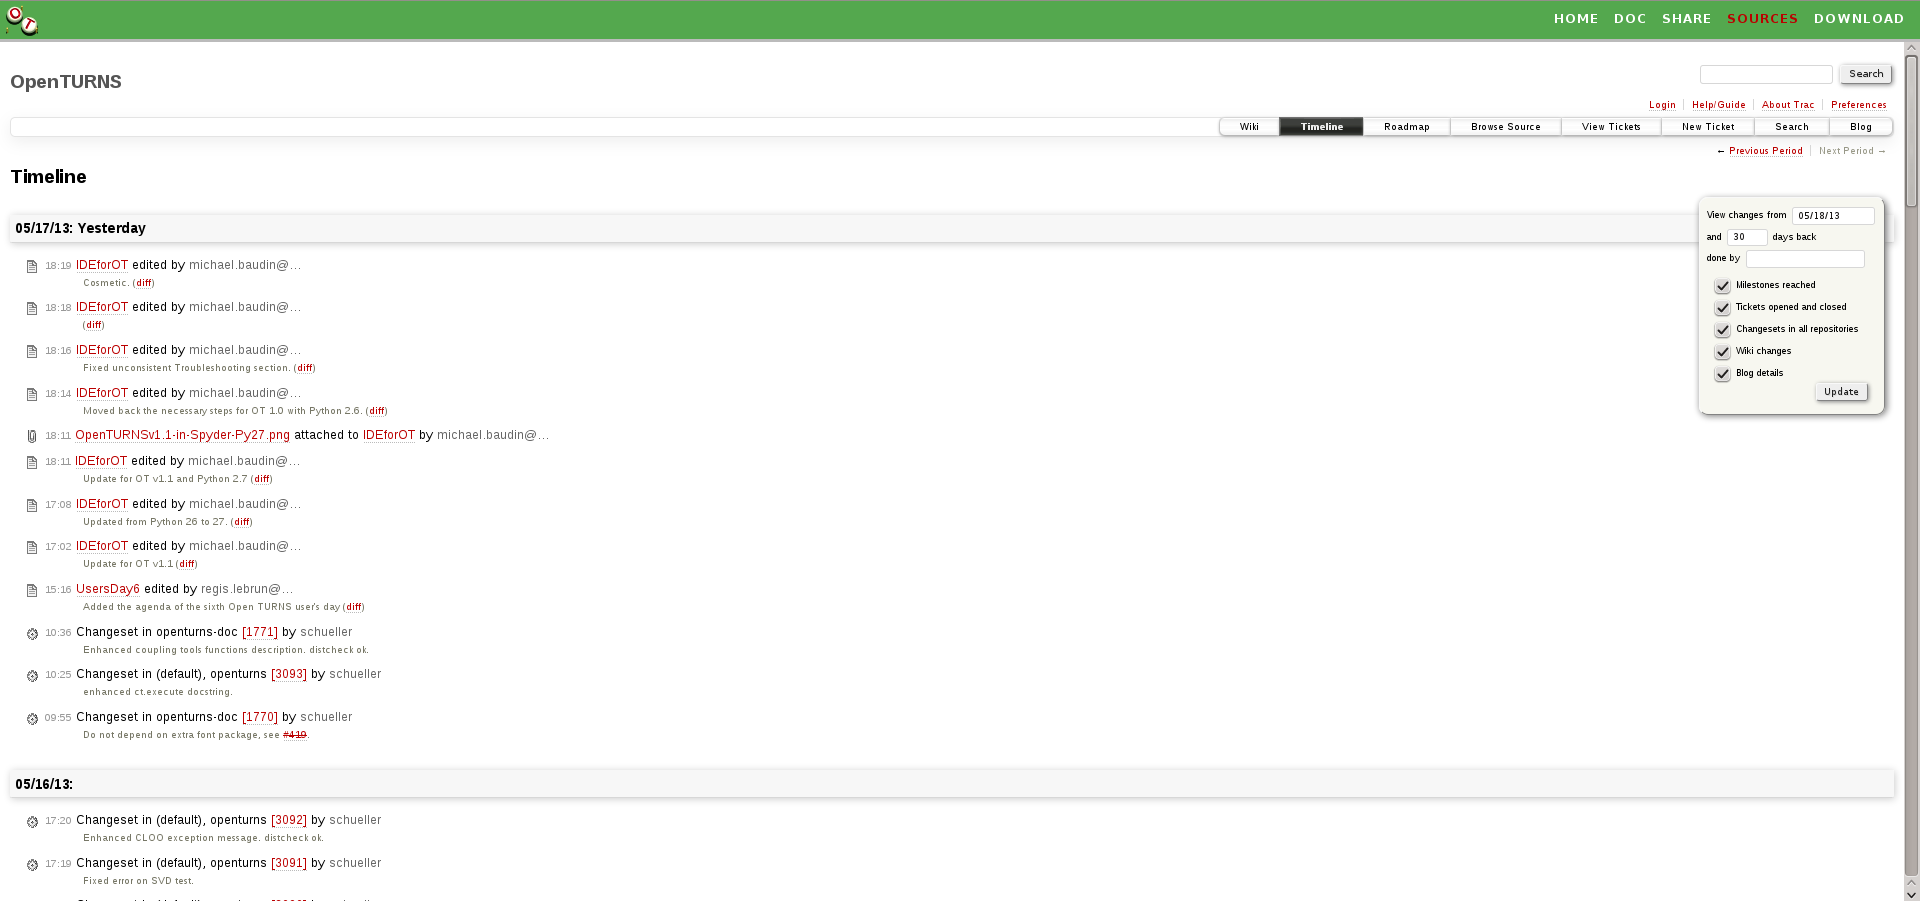
\includegraphics[scale=0.33]{Figures/Timeline.png}
\caption{Trac interface: the timeline}\label{fig:timeline}
\end{center}
\end{figure}

Trac also allows you to explore the vcs repository from your browser at \url{http://trac.openturns.org/browser}; the snapshot \ref{fig:browser} here focuses on one changeset, showing the changes in in files.

\begin{figure}[ht]
\begin{center}
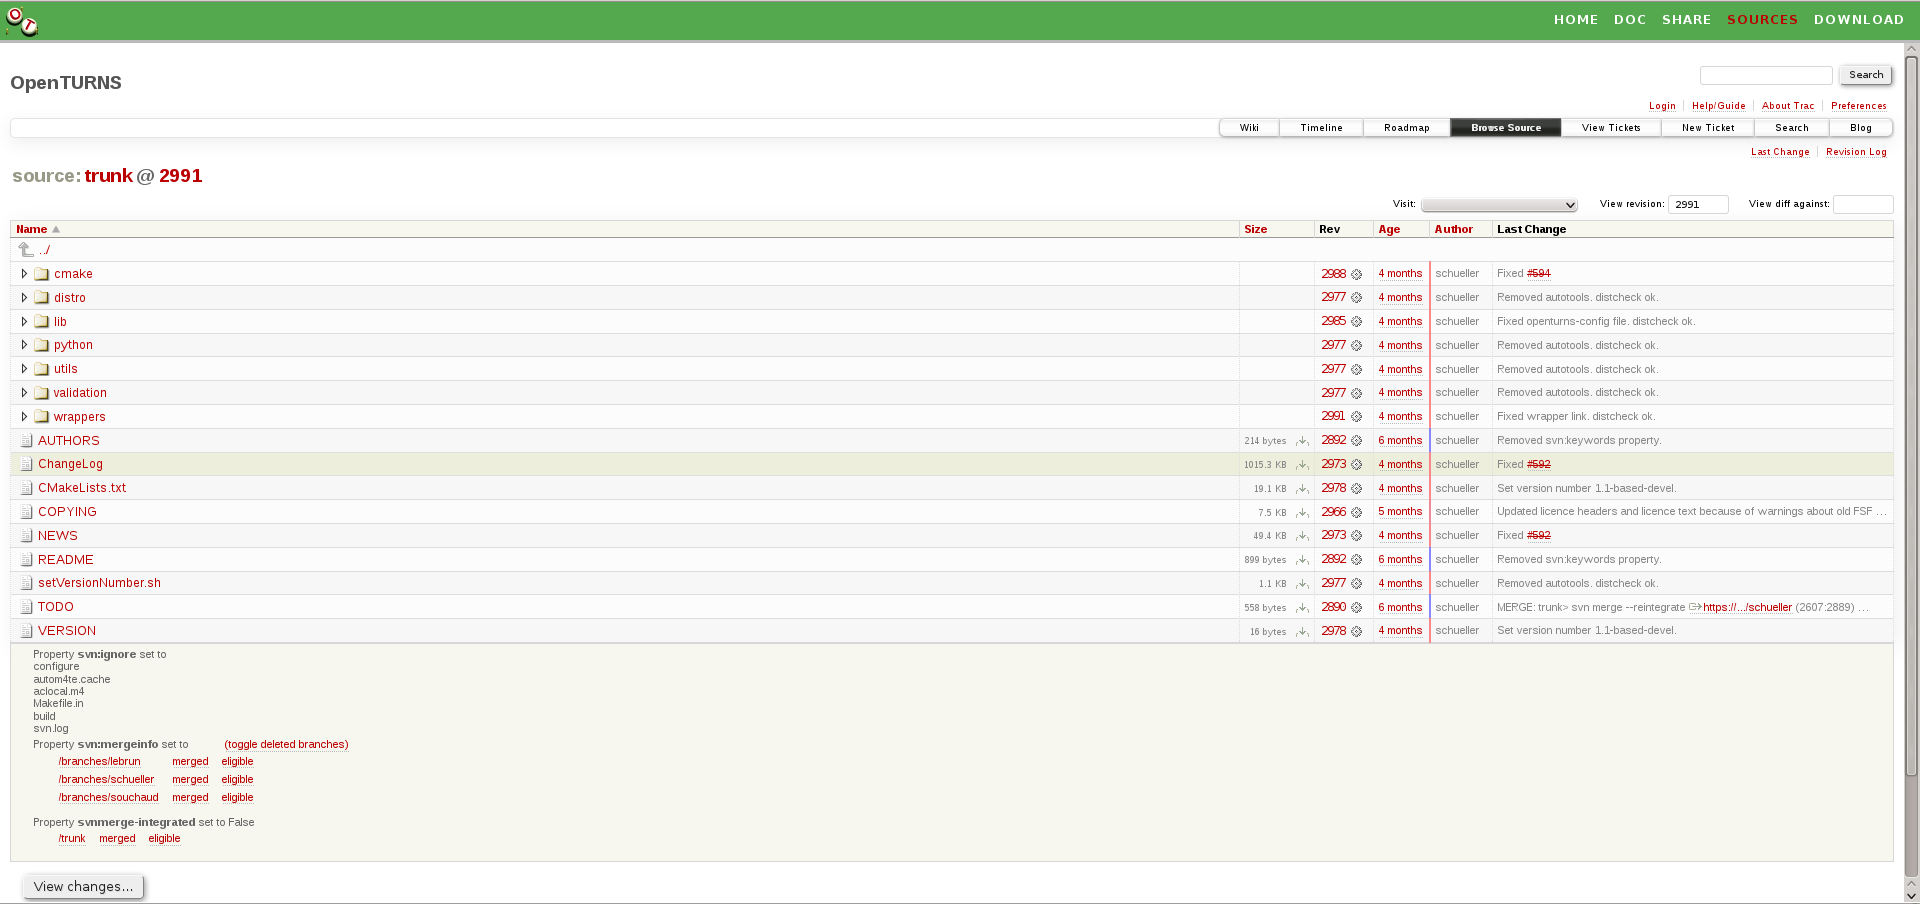
\includegraphics[scale=0.33]{Figures/BrowseSource.png}
\caption{Trac interface: the source browser}\label{fig:browser}
\end{center}

\end{figure}

Trac provides a bug-tracker at \url{http://trac.openturns.org/report}. The snapshot \ref{fig:ticket1} shows the list of active tickets.

\begin{figure}[ht]
\begin{center}
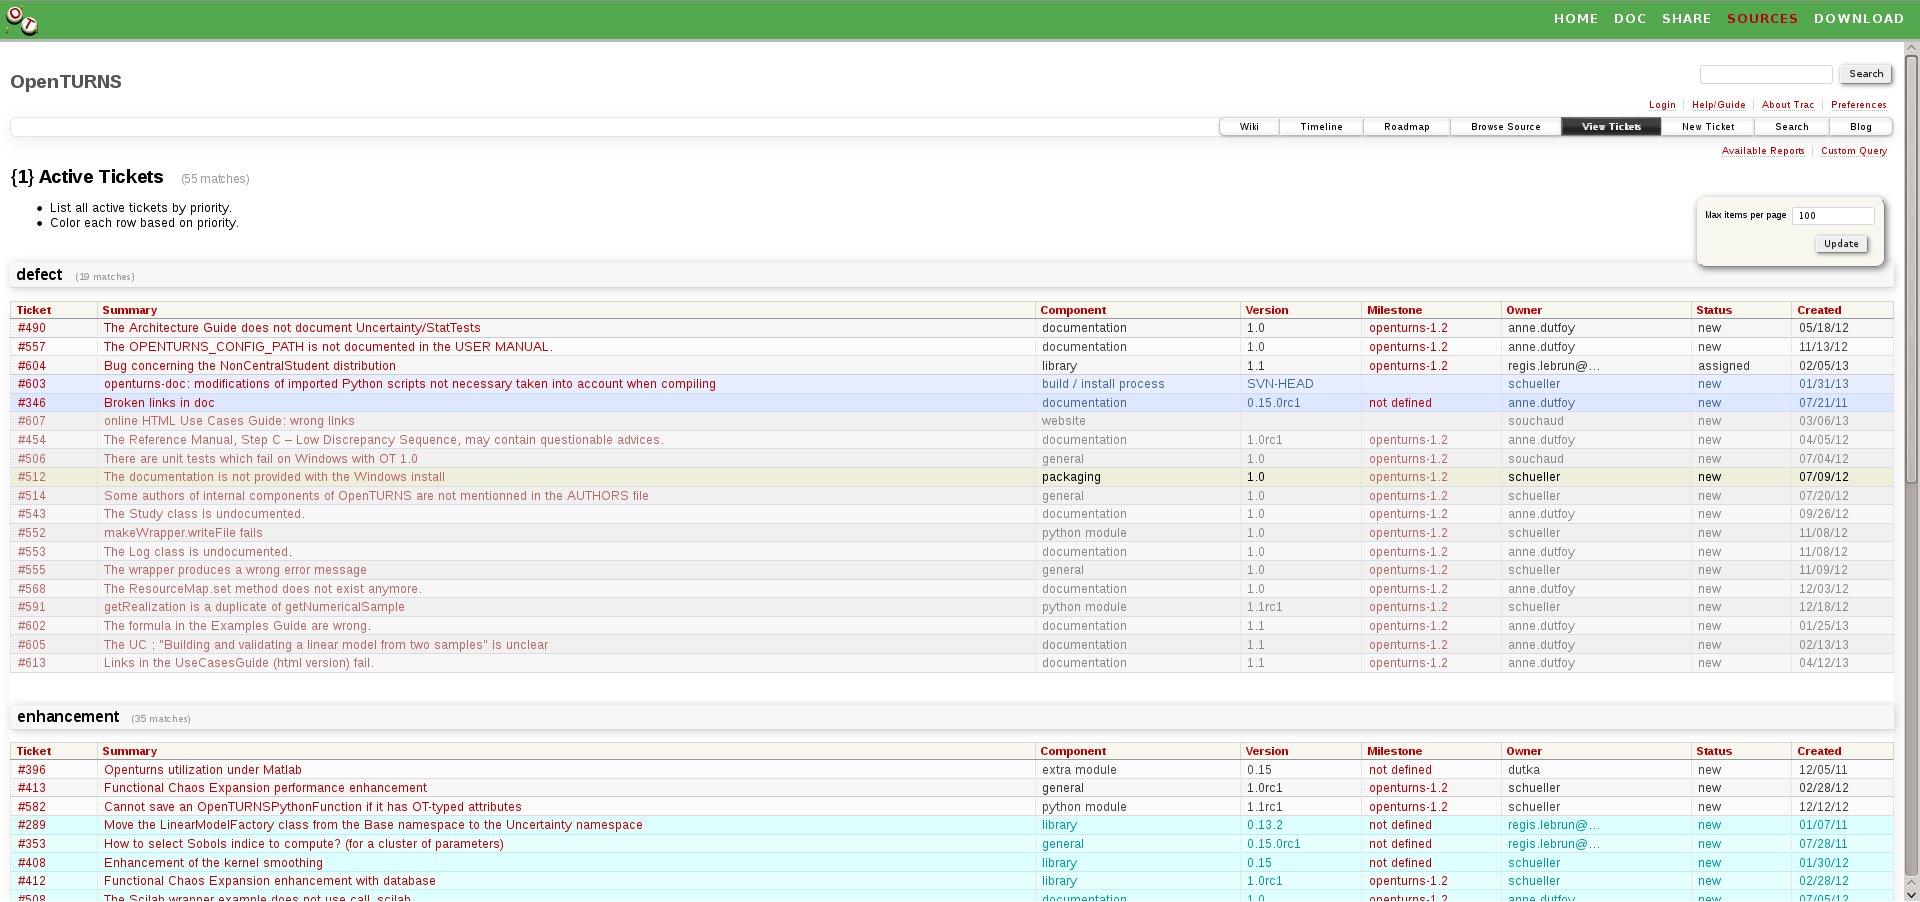
\includegraphics[scale=0.33]{Figures/Tickets1.png}
\caption{Trac interface: the ticket report view}\label{fig:ticket1}
\end{center}

\end{figure}

Each ticket features attributes to help classification, interactive comments and file attachment. Snapshot \ref{fig:ticket2} exposes the details of a ticket.

\begin{figure}[ht]
\begin{center}
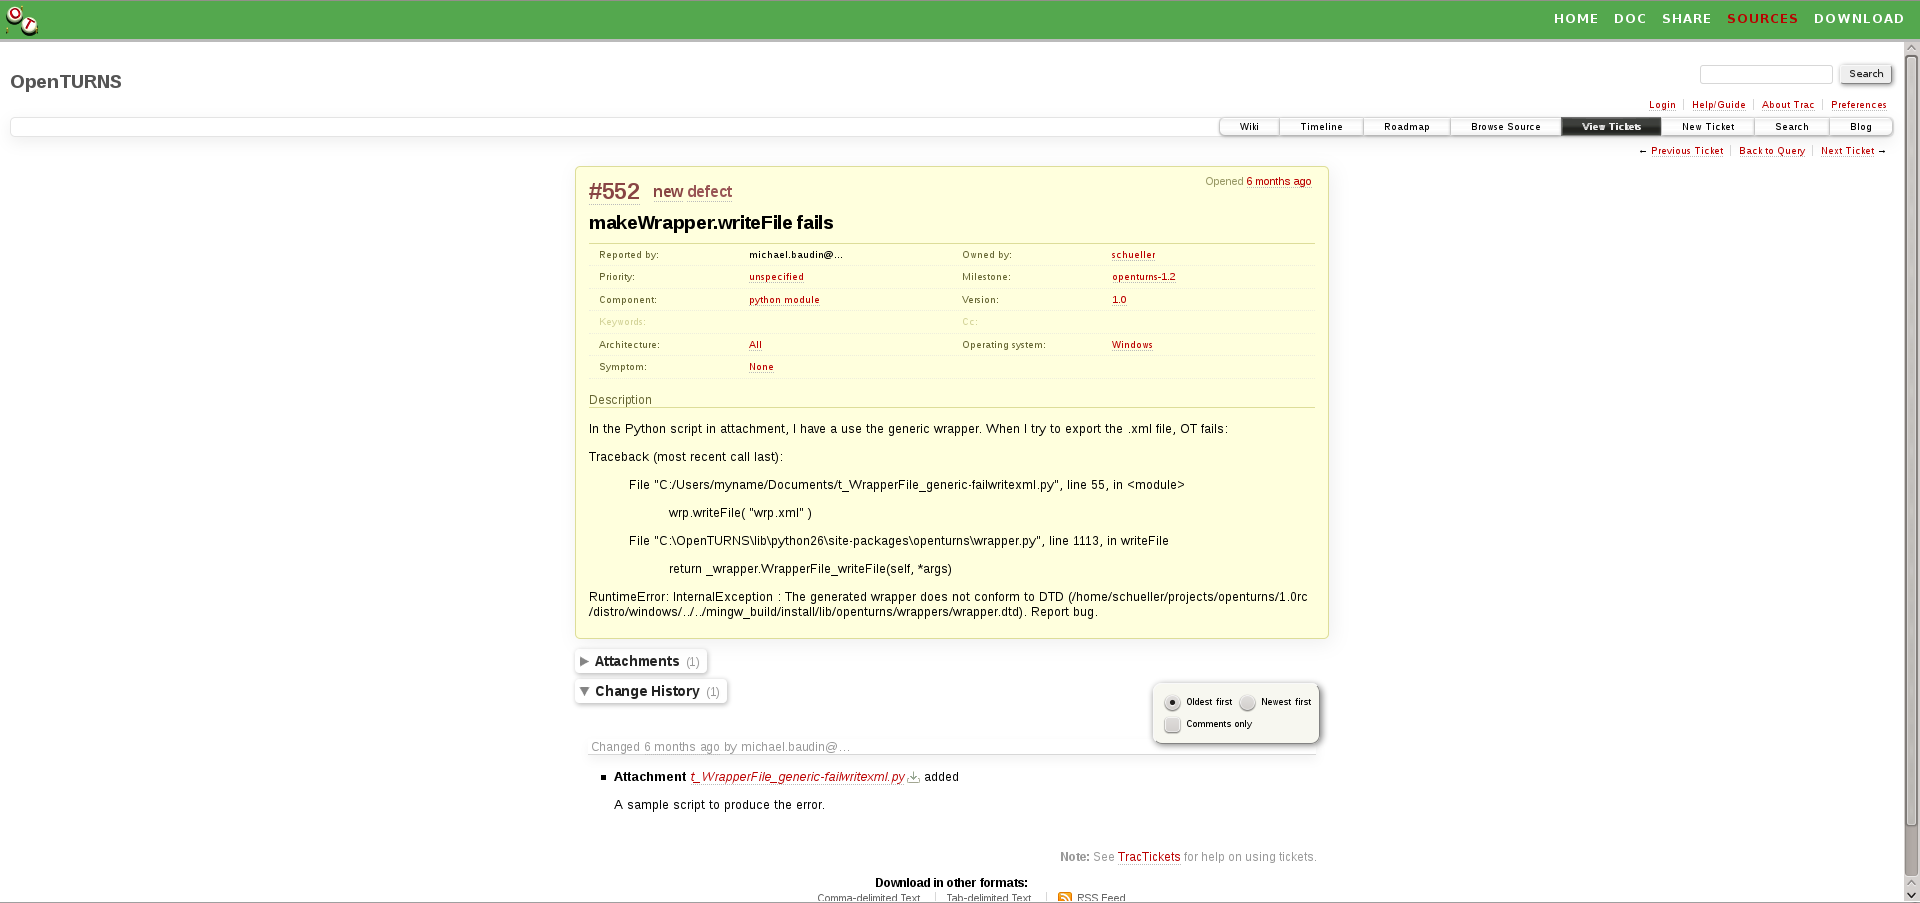
\includegraphics[scale=0.33]{Figures/Tickets2.png}
\caption{Trac interface: details of a ticket report}\label{fig:ticket2}
\end{center}
\end{figure}

\subsection{Other requirements}

\label{namespace}\subsubsection{Namespace}

All the classes of the \OT\ library are accessible within a single namespace named OT and aliased as OpenTURNS. It allows to insulate these classes from classes from another project that could share the same name. Macros are provided to enclose your code in the \OT\ namespace as follow:

\begin{lstlisting}
BEGIN_NAMESPACE_OPENTURNS
// code
END_NAMESPACE_OPENTURNS
\end{lstlisting}

\subsubsection{Internationalization}

The OpenTURNS platform is meant to be widely distributed within the scientific community revolving around probability and statistics, which is essentially an international community. Therefore, the platform should be designed so as to be adjustable to the users, particularly those who do not speak English\footnote{English has been chosen as the native language for the OpenTURNS platform.}.

This involves not using any messages directly in the source code of the platform, but rather to create a resource catalogue that can be loaded, according to the locale setting of the user, when the application is launched.

Another consequence of internationalization is the need for the Unicode extended character set to be used for all strings.

\subsubsection{Accessibility}

The OpenTURNS platform shall be accessible to disabled users. This has implications on the ergonomics and the design of the User Interface, particularly the GUI which should offer keyboard shortcuts for any available function as well as keyboard-based (rather than mouse-based) mechanisms to handle and select objects.


\subsubsection{Programming conventions}

Please refer to appendix \ref{coding_rules}.

\cleardoublepage

\section{Documentation development}
This section deals with documentation development.

\subsection{Retrieve the documentation}

\begin{enumerate}
\item Install the required tools: tralics, xsltproc and the usual latex packages.
\item Retrieve a documentation branch
  \begin{lstlisting}
    svn co https://svn.openturns.org/openturns-doc/branches/doe
  \end{lstlisting}
  \setcounter{oldenumi}{\value{enumi}}
\end{enumerate}

\subsection{Develop the documentation}
\begin{enumerate}
  \setcounter{enumi}{\value{oldenumi}}
\item Add your contribution, update the CMakeLists when adding new files.
\item Build the documentation:
  \begin{lstlisting}
    mkdir build
    cd build
    cmake -DCMAKE_INSTALL_PREFIX=$PWD/install ..
    make
  \end{lstlisting}

\item Check the PDF and HTML outputs
  \begin{lstlisting}
    make install
    xpdf install/share/doc/openturns-doc/pdf/OpenTURNS_ReferenceGuide.pdf
    firefox install/share/doc/openturns-doc/html/ReferenceGuide/index.xhtml
  \end{lstlisting}

  \setcounter{oldenumi}{\value{enumi}}
\end{enumerate}

\subsection{Run embedded scripts}
\begin{enumerate}
  \setcounter{enumi}{\value{oldenumi}}
\item Detect your openturns installation:
  \begin{lstlisting}
    cmake -DUSE_OPENTURNS=ON \
    -DOpenTURNS_DIR=<OT_PREFIX>/lib/cmake/openturns ..
  \end{lstlisting}

\item Run tests
  \begin{lstlisting}
    make check
  \end{lstlisting}
  and all the tests should be successful else check the log file test/Testing/Temporary/LastTest.log.

\end{enumerate}

\cleardoublepage

\section{Module development}
This section deals with the process of creation of a new extra module.

\subsection{Copy and adapt an existing template}

\begin{enumerate}
\item Copy and rename the source tree of an example module (for example the Strange module) from the OpenTURNS source tree. The examples modules are located under the module subdirectory of OpenTURNS source tree:
  \begin{lstlisting}
    svn export https://svn.openturns.org/openturns-modules/template/trunk MyModule
  \end{lstlisting}
\item Adapt the template to your module:
  \begin{lstlisting}
    ./customize MyModule MyClass
  \end{lstlisting}
  This command changes the module name into MyModule in all the scripts, and adapt the example class to the new name MyClass.
  \setcounter{oldenumi}{\value{enumi}}
\item Set the version of your module:
  \begin{lstlisting}
    ./setVersionNumber.sh 1.0
  \end{lstlisting}
  This command changes the module version, which is 0.0 by default.
  \setcounter{oldenumi}{\value{enumi}}
\end{enumerate}

\subsection{Develop the module}
\begin{enumerate}
  \setcounter{enumi}{\value{oldenumi}}
\item Implement your module using the same rules as described in the sections \ref{SingleClass} and \ref{WholeDirectory}.
\item Build your module as usual:
  \begin{lstlisting}
    mkdir build
    cd build
    cmake -DCMAKE_INSTALL_PREFIX=$PWD/install \
    -DOpenTURNS_DIR=OT_PREFIX/lib/cmake/openturns ..
    make
    make check
    make install
    make installcheck
  \end{lstlisting}
  \setcounter{oldenumi}{\value{enumi}}
\end{enumerate}

\subsection{Install and test}
\begin{enumerate}
  \setcounter{enumi}{\value{oldenumi}}
\item Check that you have a working OpenTURNS installation, for example by trying to load the OpenTURNS module:
  \begin{lstlisting}
    python -c "import openturns as ot; print(ot.__version__)"
  \end{lstlisting}
  and python should not complain about a non existing openturns module.

\item Test your module within python:
  Adjust your PYTHONPATH if necessary
  \begin{lstlisting}
    python
    >>> import mymodule
  \end{lstlisting}
  and python should not complain about a non existing mymodule module.

\item Create a source package of your module:
  \begin{lstlisting}
    make package_source
  \end{lstlisting}
  It will create a tarball named mymodule-X.Y.tar.gz (and mymodule-X.Y.tar.bz2), where X.Y is the version number of the module.

  That's all folks!
  \setcounter{oldenumi}{\value{enumi}}
\end{enumerate}

\cleardoublepage

\extanchor{wrapperDev}
\section{Wrapper development}
% Copyright (C) 2005-2015 Airbus - EDF - IMACS - Phimeca
% Permission is granted to copy, distribute and/or modify this document
% under the terms of the GNU Free Documentation License, Version 1.2
% or any later version published by the Free Software Foundation;
% with no Invariant Sections, no Front-Cover Texts, and no Back-Cover
% Texts.  A copy of the license is included in the section entitled "GNU
% Free Documentation License".


\subsection{Pure python wrappers}

Python wrappers aim to be an easy way for wrapping external code. The external code can be an analytical mathematical formula or a coupling involving several computational codes dedicated to the resolution of a very complex physical problem.

Python wrappers are not the best solution if your external code last less than a microseconds and if you need to resolve billions of points. In that case, for better performance, consider using the library wrapper. In any other cases, Python wrapper is the recommended choice. For further details on speed optimization see paragraph \ref{speedo}.

On OpenTURNS, two Python wrappers are available to wrap an external code:
\begin{itemize}
\item the PythonFunction is a simple monothreaded Python wrapper.
\item the DistributedPythonFunction is a Python wrapper than can launch code in parallel on the local machine or deploy it among several computers.
\end{itemize}
These two methods will be described in the following sections.


\subsubsection{PythonFunction}

A PythonFunction is a NumericalMathFunction where the \verb|_exec| or \verb|_exec_sample| function are launched in a Python interpreter.
Here is an example of how to implement it:

\inputscript{pythonfunction_point}

Some explanations of the code :
\begin{itemize}
\item[line 3-7] The \verb|compute_point| function constructs the out point from the in point. The in and out array size must correspond to the sizes set in the PythonFunction constructor. In this example, X will be an array of size 2 and Y must be an array of size 1. The output point can be a Python list, an \OT\ NumericalPoint or a Numpy array.
\item[line 9] Construct the PythonFunction by passing function reference.
\end{itemize}


The \verb|_exec_sample| function can be implemented to speedup the compute using vectorization on large sample. It receives an input sample and must return an output sample. For further details on speed optimization see paragraph \ref{speedo}. Here is an example using \verb|_exec_sample| function:

\inputscript{pythonfunction_sample}

The output sample can be a NumericalSample, a Python list of list or a Numpy array of array. This function is optional.
If \verb|_exec_sample| is not implemented and \OT\ must compute a sample, the \verb|_exec| function is called several time: once for each point of the sample. On contrary, if only \verb|_exec_sample| is given and a point must be computed, the point is inserted in a sample of size 1, computed through \verb|_exec_sample| and extracted from the result sample.


The PythonFunction is quite simple to use. When used with coupling\_tools module, it can wrap external program easily too.


\subsubsection{External code coupling tools}


\paragraph{Simple example}

Here is a simple example of wrapper where compute is made in an external program with the help of openturns.coupling\_tools module:

\inputscript{pythonfunction_couplingtools}

Some explanations of the code :
\begin{itemize}
\item[line 8] \verb|coupling_tools.replace| replace \verb|@E| and \verb|@F| occurence found in \verb|input_template.py| file and write the result to \verb|infile| file. \verb|X[0]| value will replace \verb|'@E'| token and \verb|X[1]| will replace \verb|'@F'| token.
\item[line 11] The external program is launched. The input filename is passed by parameters to the program.
\item[line 14] \verb|coupling_tools.get| get the value following  \verb|'Z='| token in \verb|output.py| file.
\end{itemize}
Template file example:

\inputscript{input_template}

External program example:

\inputscript{external_program}


\paragraph{More examples}

\subparagraph{The replace function} can edit file in place. It can format values in anyway. Actually, values can be of type "string", if not, they are converted using str() Python function:

\begin{description}
\item[Usage:] \rule{0pt}{1em}
  \begin{description}
  \item \textit{replace(infile, outfile, tokens, values, encoding=default\_encoding)}
  \end{description}
\item[Arguments:] \rule{0pt}{1em}
  \begin{description}
  \item \textit{infile}: template file that will be parsed
  \item \textit{outfile}: file that will received the template parsed. If equal to None or to \textit{infile}, the result file will be moved to infile
  \item \textit{tokens}: a list of regex that will be replaced
  \item \textit{values}: list of values (can be string, float, ...) that will replace the tokens. The list must have the same size as tokens
  \item \textit{encoding}: the file encoding, as string, i.e. ascii, latin\_1, utf\_8, ...
  \end{description}
\end{description}
\bigskip


\begin{lstlisting}
  replace(outfile='input_template.py', infile=None,
  tokens=['@E', '@F'], values=['%.2f' % 5.2569, 'toto'])
\end{lstlisting}


\begin{lstlisting}
  replace(outfile='input_template.py', infile=None,
  tokens=['@E', '@F'], values=['%.2f' % 5.2569, 'toto'])
\end{lstlisting}

The input\_template.py file will then be modify like this :
\begin{lstlisting}
  E=5.25
  F=toto
\end{lstlisting}

Be careful with overlapping tokens:
\begin{lstlisting}
  # if input_template.py = 'E=@E EE=@EE')
  replace(infile="input_template.py",
  outfile="None",
  tokens=["@E", "@EE"],
  values=[1, 2])
  # => raise exception!! -> @EE token not found!
  # (this is due to the first pass with token "@E" that modify
  # "input_template.py" like this : 'E=1 EE=1E')
\end{lstlisting}

Solution to overlapping tokens: put longest tokens first:
\begin{lstlisting}
  # template.in = 'E=@E EE=@EE')
  replace(infile="template.in",
  outfile="prgm_data.in",
  tokens=["@EE", "@E"],
  values=[2, 1])
  # => prgm_data.in = 'E=1 EE=2')
\end{lstlisting}


\subparagraph{The execute function} can launch an external code.

\begin{description}
\item[Usage:] \rule{0pt}{1em}
  \begin{description}
  \item \textit{execute(cmd, workdir=None, is\_shell=False, shell\_exe=None, hide\_win=True,
    check\_exit\_code=True, get\_stdout=False, get\_stderr=False)}
  \end{description}

\item[Arguments:] \rule{0pt}{1em}
  \begin{description}
  \item \textit{cmd}: a string representing the command. e.g.: 'ls -l /home'
  \item \textit{workdir}: set the current directory of the executed command
  \item \textit{is\_shell}: if set to True, the command is started in a shell (bash). default: False.
  \item \textit{shell\_exe}: path to the shell. e.g. /bin/zsh. default: None: /bin/bash.
  \item \textit{hide\_win}: hide cmd.exe popup on windows
  \item \textit{check\_exit\_code}: if set to True: raise a RuntimeError exception if return code of process != 0
  \item \textit{get\_stdout}: whether standard output of the command is returned
  \item \textit{get\_stderr}: whether standard error of the command is returned
  \end{description}

\item[Value:] \rule{0pt}{1em}
  \begin{description}
  \item the exit code of the command
  \item the stdout data if get\_stdout parameter is set
  \item the stderr data if get\_stderr parameter is set
  \end{description}

\end{description}
\bigskip

\subparagraph{The get\_value function}\label{getvalue} can deal with several type of output file.


\begin{description}
\item[Usage:] \rule{0pt}{1em}
  \begin{description}
  \item \textit{get\_value(filename, token=None, skip\_token=0, skip\_line=0, skip\_col=0, encoding=default\_encoding)}
  \end{description}
\item[Arguments:] \rule{0pt}{1em}
  \begin{description}
  \item \textit{filename}: a file that will be parsed
  \item \textit{token}: a regex that will be searched. The value right after the token is returned. Default: None (no token searched)
  \item \textit{skip\_token}: the number of tokens that will be skipped before getting the
    value. If set to != 0, the corresponding token parameter must not be
    equal to None.
    If skip\_tokens < 0: count tokens backward from the end of the file.
    Default: 0: no token skipped
  \item \textit{skip\_line}: number of lines skipped from the token found.
    If corresponding token equal None, skip from the beginning of the file.
    If corresponding token != None, skip from the token.
    If skip\_line < 0: count lines backward from the token or from the end
    of the file. Be careful: a last empty line is taken into account too.
    Default: 0: no line skipped
  \item \textit{skip\_col}: number of columns skipped from the token found.
    If corresponding token = None, skip words from the beginning of the line.
    If corresponding token != None, skip words from the token.
    If skip\_col < 0: count col backward from the end of the line or from
    the token.
    Default: 0: no column skipped
  \item \textit{encoding}: the file encoding, as string, i.e. ascii, latin\_1, utf\_8, ...
  \end{description}

\item[Value:] \rule{0pt}{1em}
  \begin{description}
  \item a real value
  \end{description}
\end{description}
\bigskip




\begin{itemize}
\item content of the results.out file used for the following examples
  \begin{lstlisting}
    1  2  3  04  5  6
    7  8  9  10
    11 12 13 14

    @Y1= 11.11celcius
    @Y2= -0.89
    @Y1= 22.22
    @Y1= 33.33

    line1: 100 101 102
    line2: 200 201 202
    line3: 300 301 302
  \end{lstlisting}
\item search token, the value right after the token is returned: \\
  \begin{lstlisting}
    Y = get_value('results.out', token='@Y1=') # 11.11
  \end{lstlisting}
\item skip lines and columns (useful for array search):\\
  \begin{lstlisting}
    get_value('results.out', skip_line=1, skip_col=2) # 9
  \end{lstlisting}
\item skip lines and columns backward (be careful: if there is an empty line at the end of the file, it is taken into account. i.e. this last empty line will be reached using skip\_line=-1):\\
  \begin{lstlisting}
    get_value('results.out', skip_line=-2, skip_col=-2) # 201
  \end{lstlisting}
\item search the 3rd appearance of the token:\\
  \begin{lstlisting}
    get_value('results.out', token='@Y1=', skip_token=2) # 33.33
  \end{lstlisting}
\item search the 2nd appearance of the token from the end of the file:\\
  \begin{lstlisting}
    get_value('results.out', token='@Y1=', skip_token=-2) # 22.22
  \end{lstlisting}
\item search a token and then skip lines and columns from this token:\\
  \begin{lstlisting}
    get_value('results.out', token='@Y1=', skip_line=5, skip_col=-2) # 101
  \end{lstlisting}
\item search the 2nd token and then skip lines and columns from this token:\\
  \begin{lstlisting}
    get_value('results.out', token='@Y1=', skip_token=1, skip_line=5, skip_col=1) # 300
  \end{lstlisting}
\end{itemize}

\subparagraph{The get function} works actually the same way the get\_value function do, but on several parameters:\\

\begin{description}
\item[Usage:] \rule{0pt}{1em}
  \begin{description}
  \item \textit{get(filename, tokens=None, skip\_tokens=None, skip\_lines=None, skip\_cols=None, encoding=default\_encoding)}
  \end{description}

\item[Arguments:] \rule{0pt}{1em}
  \begin{description}
  \item \textit{filename}: a file that will be parsed
  \item \textit{tokens}: see \ref{getvalue} function
  \item \textit{skip\_tokens}: see \ref{getvalue} function
  \item \textit{skip\_lines}: see \ref{getvalue} function
  \item \textit{skip\_cols}: see \ref{getvalue} function
  \item \textit{encoding}: the file encoding, as string, i.e. ascii, latin\_1, utf\_8, ...
  \end{description}

\item[Value:] \rule{0pt}{1em}
  \begin{description}
  \item a list of real values.
  \end{description}
\end{description}
\bigskip

\begin{lstlisting}
  get('results.out', tokens=['@Y1=', '@Y2'], skip_lines=[5, 0], skip_cols=[-2, 0]) # [101, -0.89]
\end{lstlisting}


\subparagraph{The get\_regex function} parses the outfile the same way as \OT\ LibraryWrapper do. It is provided for backward compatibility:\\

\begin{description}
\item[Usage:] \rule{0pt}{1em}
  \begin{description}
  \item \textit{get\_regex(filename, patterns)}
  \end{description}

\item[Arguments:] \rule{0pt}{1em}
  \begin{description}
  \item \textit{filename}: the file to parse
  \item \textit{patterns}: a list of patterns that will permit to get the values.
    \textbackslash \textbackslash R and \textbackslash \textbackslash I can be used to match float and integer.
    \textbackslash \textbackslash s can be used to match any whitespace character (= [ \textbackslash \textbackslash t\textbackslash \textbackslash n\textbackslash \textbackslash r\textbackslash \textbackslash f\textbackslash \textbackslash v])
    \textbackslash \textbackslash S can be used to match any non-whitespace character.
    The value to be searched must be surrounded by '(' and ')' (see example).
  \end{description}

\item[Value:] \rule{0pt}{1em}
  \begin{description}
  \item a list of values corresponding to each pattern.
    If nothing has been found, the corresponding value is set to None.
  \end{description}
\end{description}
\bigskip



\begin{lstlisting}
  Y = get_regex('results.out', patterns=['@Y2=(\R)']) # -0.89
\end{lstlisting}


\paragraph{Reference}

Most up to date coupling tools module documentation is available through docstring in Python console:

\begin{lstlisting}
  import openturns as ot
  help(ot.coupling_tools.get_value)
\end{lstlisting}

Or in IPython console:
\begin{lstlisting}
  ot.coupling_tools.replace?
\end{lstlisting}



\cleardoublepage

\subsection{Library wrappers}

The library wrapper allows to launch calculus in a multi-threaded context.

\subsubsection{C++ library wrapper}

This is the most low-level wrapper available.
Due to being compiled, it allows for very low-latency.
However, beware that the development process is quite difficult.
We discourage it as python wrappers should fit your needs in most cases.
Refer to appendix \ref{library_wrapper} for further instructions.

\subsubsection{Generic wrapper}

The 'generic' wrapper relies on the base library wrapper, but is usable from Python. It and was an effort to simplify it's use before the work on the pure python distributed wrapper module existed. Unlike DistributedPythonFunction, it does not allow distributed computation over remote hosts, and is less customizable. This wrapper requires the list of variables, the list of files involved in the communication with the external code, and the execution parameters.

\paragraph{Variables}

The variables are represented by list of dictionaries, and each of them may contains the following keys:
\begin{itemize}
\item id\_: variable name as string
\item comment\_: a comment to inform on the variable
\item unit\_: the unit which the variable is expressed in
\item regexp\_: find regex, as string
\item format\_: output regex, as string
\item type\_: the type of the variable (input or output), as integer:
  \begin{itemize}
  \item WrapperDataFileType.IN, or string 'in': input variable (default)
  \item WrapperDataFileType.OUT, or string 'out': output variable
  \end{itemize}
\item fromType\_: The type of the from\_ member:
  \begin{itemize}
  \item WrapperDataVariableLocation.LINE: the location is a line number
  \item WrapperDataVariableLocation.REGEXP: the location is a regular expression
  \end{itemize}
\item from\_: the location where substitution should start, as string
\item toType\_: The type of the to\_ member:
  \begin{itemize}
  \item WrapperDataVariableLocation.LINE: the location is a line number
  \item WrapperDataVariableLocation.REGEXP: the location is a regular expression
  \end{itemize}
\item to\_: the location where substitution should stop, as string
\end{itemize}

\paragraph{Coupling files}

The coupling files are represented by a list of dictionaries, each of them may contain the following fields:
\begin{itemize}
\item id\_: the id of the file (any string to distinguish each file from another)
\item name\_: the name of the file (stdin, stdout, log, etc.), as string
\item path\_: the path of the file (/tmp/stdin, /var/log/mylog, etc.), as string
\item subst\_: the list of variable's ids to be substituted in the file, as string, e.g. 'E,L'
\item type\_: the type of the file (input or output):
  \begin{itemize}
  \item WrapperDataFileType.IN: the file is an input file
  \item WrapperDataFileType.OUT: the file is an output file
  \end{itemize}
\end{itemize}

\paragraph{Execution parameters}

The execution parameters are represented by a dictionary with the following fields:
\begin{itemize}
\item state\_: the sharing mode of internal state, as integer:
  \begin{itemize}
  \item WRAPPER\_SHAREDSTATE (default)
  \item WRAPPER\_SPECIFICSTATE
  \end{itemize}
  % \item mode\_: the mode of invocation of the external code, as integer:
  %   \begin{itemize}
  %   \item WRAPPER\_STATICLINK (default)
  %   \item WRAPPER\_DYNAMICLINK
  %   \item WRAPPER\_FORK
  %   \end{itemize}
\item in\_: the transmission mode for input arguments, as integer:
  \begin{itemize}
  \item WRAPPER\_FILES (default)
  \item WRAPPER\_PIPE
  \item WRAPPER\_ARGUMENTS
  \item WRAPPER\_SOCKET
  \item WRAPPER\_CORBA
  \end{itemize}
\item out\_: the transmission mode for output arguments, same as above
\item command\_: the command that should invoque the external code according to mode, as string
\item userPrefix\_: the prefix that helps the user to find its compute dir, as string
\end{itemize}

\paragraph{Wrapper instanciation}

Once the variable list, file list, and execution parameters are ready, they are passed on to the makeWrapper function. The makeWrapper function builds a WrapperFile object which can be provided as an argument to NumericalMathFunction. The writeFile method of WrapperFile can be used to ouput the XML representation of the wrapper. Here is an example of wrapper script from the automatic tests:

\begin{lstlisting}
  # Variables
  vars = ({ "id_" : "F",
    "type_" : "in",
    "regexp_" : "^\S*F\S*=\S*\R\S*$",
    "format_" : "F=%20.13G"  },

    { "id_" : "E",
      "type_" : "in",
      "regexp_" : "^\S*E\S*=\S*\R\S*$",
      "format_" : "E=%20.13G"  },

      { "id_" : "Z",
        "type_" : "out",
        "regexp_" : "^\S*Z\S*=\S*(\R)\S*$" },
      )

      # Files
      files = ({ "id_" : "infile",
        "type_" : "in",
        "path_" : "inFILE_generic",
        "subst_" : "E,F"  },

      { "id_" : "outfile",
        "type_" : "out",
        "path_" : "outFILE_generic",
        "subst_" : "Z"    },
      )

      # Parameters
      params = {
        "command_" : sys.executable + " -c \"exec(compile(open('inFILE_generic').read(), 'inFILE_generic', 'exec')); Z=E*F; print('Z=' + str(Z))\" > outFILE_generic",
        "userPrefix_" : "GenericWrapperTest"}

      wrp = makeWrapper( vars, files, params )
      wrp.writeFile( "wrp.xml" )
      model = NumericalMathFunction( wrp )
\end{lstlisting}

and its the corresponding XML representation:
\begin{lstlisting}
  <?xml version="1.0" encoding="UTF-8"?>
  <wrapper version="1">
  <library>
  <path>generic.so</path>
  <description>
  <variable-list>
  <variable id="F" type="in">
  <regexp>^\S*F\S*=\S*\R\S*$</regexp>
  <format>F=%20.13G</format>
  </variable>
  <variable id="E" type="in">
  <regexp>^\S*E\S*=\S*\R\S*$</regexp>
  <format>E=%20.13G</format>
  </variable>
  <variable id="Z" type="out">
  <regexp>^\S*Z\S*=\S*(\R)\S*$</regexp>
  </variable>
  </variable-list>
  <function provided="yes">generic</function>
  <gradient provided="no"></gradient>
  <hessian provided="no"></hessian>
  </description>
  </library>
  <external-code>
  <data>
  <file id="infile" type="in">
  <path>inFILE_generic</path>
  <subst>E,F</subst>
  </file>
  <file id="outfile" type="out">
  <path>outFILE_generic</path>
  <subst>Z</subst>
  </file>
  </data>
  <wrap-mode type="static-link" state="shared">
  <in-data-transfer mode="files"/>
  <out-data-transfer mode="files"/>
  </wrap-mode>
  <command>/usr/bin/python -c "exec(compile(open('inFILE_generic').read(), 'inFILE_generic', 'exec')); Z=E*F; print('Z=' + str(Z))" &gt; outFILE_generic</command>
  <user-prefix>GenericWrapperTest</user-prefix>
  </external-code>
  </wrapper>
\end{lstlisting}
Note that illegal characters according to the XML specification, like the '\textgreater' in the original command line, are replaced by their corresponding XML entities.


\subsection{Performance considerations\label{speedo}}

Two differents cases can be encounter when wrapping code: the wrapping code is an analytical mathematical formula or it is an external code (an external process).

\subsubsection{Analytical formula}

A benchmark involving the differents wrapping methods available from \OT\ has been done using a dummy Analytical formula.


\paragraph{Benchmark sources} Optimizations of any parts of this benchmark are welcome.

\begin{itemize}
\item Benchmark of PythonFunction using \_exec function:
  \begin{lstlisting}
    big_sample = ot.Normal(2).getSample(1000*1000)
    import openturns as ot

    def _exec( X ):
    return [math.cos(pow(X[0]+1, 2)) - math.sin(X[1])]

    model = ot.PythonFunction(2, 1, _exec)
    # start timer
    out_sample = model( big_sample )
    # stop timer
  \end{lstlisting}

\item Benchmark of PythonFunction using \_exec\_sample function:
  \begin{lstlisting}
    def _exec_sample( Xs ):
    import numpy as np
    XsT = np.array(Xs).T
    return np.atleast_2d(np.cos(np.power(xT[0]+1, 2)) - np.sin(xT[1])).T

    model = ot.PythonFunction(2, 1, func_sample=_exec_sample)
  \end{lstlisting}

\item Benchmark of Analytical (MuParser) function:
  \begin{lstlisting}
    model = ot.NumericalMathFunction( ('x0','x1'), ('y',),
    ('cos((x0+1) ^ 2) - sin(x1)',) )
  \end{lstlisting}

\item Benchmark of LibraryWrapper:
  \begin{lstlisting}
    model = ot.NumericalMathFunction( 'wcode' )
  \end{lstlisting}
  myCFunction.c:
  \begin{lstlisting}
    #include <math.h>
    int myCFunction( const double * X, unsigned long N,
    double * Y, unsigned long P )
    {
      Y[0] = cos(pow(X[0]+1, 2)) - sin(X[1]);
      return 0;
    }
  \end{lstlisting}
\end{itemize}


The benchmark is done on a bi XEON E5520 (Nehalem 16*2.27GHz, HT activated) with 12Go RAM.


\paragraph{Benchmark results}:

The sample containing 1 million of points is allocated in 0.282s.

\begin{tabular}{lll}
  wrapper type & time & comparison with fastest wrapper \\
  PythonFunction \_exec & 7.1s & x157 \\
  PythonFunction \_exec\_sample & 1.3s & x30 \\
  Analytical (MuParser) & 0.43s & x10 \\
  LibraryWrapper & 0.045s & x1 \\
  LibraryWrapper monothreaded & 0.1s & x2.2 \\
\end{tabular}

The previous results are linear to the size of the sample (e.g. LibraryWrapper takes 0.45s with a sample of size 10 millions).

\begin{itemize}
\item The LibraryWrapper is the fastest. The parallel version speedup is not really good for an unknown reason: on a 16 HT core machines the multithreaded version is only 2.2 times faster than the monothreaded one.

  \OT\ parallelize LibraryWrapper function using TBB or PThreads. TBB implementation is 30\% faster than PThread one. This benchmark has been done using the TBB implementation (\OT\ choose it by default). Note that the LibraryWrapper parallelization could be in the future improved by using MPI.

\item MuParser is the 2nd fastest (10 times slower than the first).

  The MuParser library embedded in \OT\ is not multithreaded. Embedding a parallel version of MuParser could give better results. But if the LibraryWrapper is forced to be executed on 1 core, it is still 4 times faster that the MuParser.
\item Using an optimized \_exec\_sample python function through numpy gives better results (6x faster) than a simple \_exec python function, but it is still much slower than the compiled library (30 times slower).

  Note that neither Python nor NumPy are multithreaded.
\end{itemize}


\paragraph{Conclusion} PythonFunction is the easiest and more adaptable wrapper but it's the slowest too. So, if you need to compute samples containing less than a million of points, PythonFunction is the good choice as the speed difference between wrappers will not be noticeable: every wrappers will compute the sample in less than a second. Otherwise choose MuParser or Library Wrapper.




\subsubsection{External process}

\paragraph{Normal program}

For usual program (compute time of 1s and above), inner wrapper complexity/overhead are not an issue cause the external program compute time will be the main part of the whole compute time. Sample can be computed faster by launching this external program in parallel.

\begin{itemize}
\item PythonFunction can not launch the \_exec function in parallel.
\item LibraryWrapper using fork mode can launch the external program on each core of the local Machine.
\item the DistributedPythonFunction from otdistfunc module can launch external program on each core of the local Machine or on each core of several remote machine.
\end{itemize}

The DistributedPythonFunction is the best choice as it combine the ease of use of Python with the ability to deploy compute on a cluster of computers.



\paragraph{Tiny program}

If the external process compute time is really fast (< 0.1s), \OT\ wrapper point's launch time (overhead) becomes important.

If performance are an issue, one should first consider that the external process is perhaps fast because it does something simple: can it be easily reimplemented in Python? If the code is not too complex, execute Python code inside a PythonFunction is usually much faster than the time to start the external process (~1000x). Here is a naive example of external process (scilab) vs PythonFunction.

\begin{itemize}
\item The following scilab script takes 0.07s per point:

  \verb|$ scilab -nb -nwni -f code.sce|

  \begin{lstlisting}
    // code.sce
    exec("input.data", -1)
    y = x1 + x2;
    f = mopen("result.data", "wt");
    mfprintf(f, "y = %.20e", y);
    file("close", f);
    quit
  \end{lstlisting}


\item Conversion to Python of the scilab script. It takes now 0.00001s per point:

  \begin{lstlisting}
    def _exec( X ):
    return X[0] + X[1]
    model = ot.PythonFunction(2, 1, _exec)
  \end{lstlisting}
\end{itemize}

If you still need to launch tiny external process, slow overhead and parallel ability are the important factors of the wrapper.
Comparison of the differents wrapper compute time with a sample of size 1000 and an external code that last 0.07s per point on a 8 cores computer:

\begin{itemize}
\item PythonFunction overhead is really slow (0.000004s) but can not launch the \_exec function in parallel.

  $(0.000004+0.07)*1000 => 70s$
\item DistributedPythonFunction overhead is near 0.05s and can launch external program in parallel.

  $(0.05+0.07)*1000 (/8core) => 15s$
\item LibraryWrapper using fork mode overhead is near 0.01s per point and can launch external program in parallel.

  $(0.01+0.07)*1000 (/8core) => 10s$

\item PythonFunction that reimplement the external program.

  $(0.00001)*1000 => 0.01s$

\end{itemize}

The LibraryWrapper is the fastest with external code that last less than 0.1s. But if possible, first consider to reimplement directly in the wrapper the tiny external code.

\cleardoublepage

\appendix

\section{Coding rules}
\newcounter{Rulecounter}
\setcounter{Rulecounter}{1}

\newcommand{\Rule}[2]{
\begin{description}
\item[{\color{blue} R\arabic{Rulecounter}}] \label{rule:#1}#2
\end{description}
\refstepcounter{Rulecounter}
}
% \newcounter{Rulecounter}
%
% \newcommand{\Rule}[2]{
% \begin{description}
% \refstepcounter*{Rulecounter}\label{rule:#1}
% \item[{\color{blue} R\arabic{Rulecounter}}] #2
% \end{description}
% }
\newcommand{\RuleX}[2]{
\begin{description}
\item[{\color{blue} R#1}] #2
\end{description}
}


\label{coding_rules}


\subsection{Introduction}
% Copyright 2005-2016 Airbus-EDF-IMACS-Phimeca
% Permission is granted to copy, distribute and/or modify this document
% under the terms of the GNU Free Documentation License, Version 1.2
% or any later version published by the Free Software Foundation;
% with no Invariant Sections, no Front-Cover Texts, and no Back-Cover
% Texts.  A copy of the license is included in the section entitled "GNU
% Free Documentation License".

\emph{We would like to thank Vincent Lefebvre and Olivier Morvant from the Descartes project, who are the original authors of this document that we have almost entirely drawn upon.}

\subsubsection{Document goals}
The coding rules proposed in this document mainly regard:
\begin{itemize}
\item the structure of modules and classes;
\item the names of the source files;
\item the use of the C++ and Python programming languages;
\item the documentation included inside the source files;
\item the format used to write statements in the programming languages.
\end{itemize}

The purpose of these rules is to provide a common formalism for the project in order to help the developers produce code that is globally homogeneous, readable, understandable by all and also efficient and reliable, respecting the architectural choices and constraints established to produce the code of the \OT\ project. The scope of this document only embraces files produced in the \OT\ project and does not apply to external software included in the project \emph{as is}.

\subsubsection{Conventions}
This paragraph establishes the conventions used in this document.

Each coding rules is identified by a unique number prefixed by the letter R.
\RuleX{xx}{Description of rule}
Examples of source code in C++ and Python are framed. Correct examples are given in blue, while incorrect examples are in red.

\lstset{language=C++, basicstyle=\normalsize}
\begin{lstlisting}[frame=TRL]
<Example>
...
\end{lstlisting}
\lstset{language=C++, basicstyle=\color{blue}}
\begin{lstlisting}[frame=RL]
<correct example>
...
\end{lstlisting}

\lstset{language=C++, basicstyle=\color{red}}
\begin{lstlisting}[frame=RLB]
<incorrect example>
...
\end{lstlisting}

When an example requires comments, these are given above the said example and they appear in italics.

\emph{Comment about example}
\lstset{language=C++, basicstyle=\normalsize}
\begin{lstlisting}[frame=TRBL]
<Example>
\end{lstlisting}

Elements from the text, rules or source code cited as an example and appearing between the two characters {\bf \textless} and {\bf \textgreater} correspond to a description of the expected items or objects. The following example shows that {\bf \textless condition \textgreater} represents a boolean expression and the function {\bf compute} is called on a piece of data of type length, with its default unit.

\begin{lstlisting}[frame=TRBL]
if ( <condition> ) {
r = compute( <length in cm> )
}
\end{lstlisting}

By extension, the following symbols are used to describe a grammar, a call syntax, etc.

\begin{tabular}{rl}
{\bf \textless real \textgreater} & a real number \\
{\bf \textless integer \textgreater} & an integer \\
{\bf \textless string \textgreater} & a string \\
{\bf \textless filename \textgreater} & a string representing a filename
\end{tabular}

The first rule is given below this introductory paragraph and deals with the language used in the code.
\Rule{Coding language}{{\bf Coding language:} the language used to program classes, functions and modules in \OT\ is English. The comments included in the source code shall be written in English as well.}

\cleardoublepage

\subsection{Package structure}
% Copyright 2005-2016 Airbus-EDF-IMACS-Phimeca
% Permission is granted to copy, distribute and/or modify this document
% under the terms of the GNU Free Documentation License, Version 1.2
% or any later version published by the Free Software Foundation;
% with no Invariant Sections, no Front-Cover Texts, and no Back-Cover
% Texts.  A copy of the license is included in the section entitled "GNU
% Free Documentation License".

In order to structure the code of the \OT\ project, the various elements (classes, functions, libraries, data) are logically organized in packages. This chapter describes the rules to be followed for the definition, management and use of these packages.

\subsubsection{Packages}
The \OT\ code is mainly located in a single library. This library is organized as a set of modules. However, there may be several interacting libraries in the future.\\
The \OT\ library is interfaced with Python through a Python module exposing almost all the \OT\ classes and operators.
\Rule{Library_independence}{Libraries at the same level are independent from each other.
The source files of a function or a class can not be shared among several modules. If two libraries share the same functions or classes, these must be grouped in a common "utility" library, in order to avoid cyclic references and dependencies.}

\Rule{C++-modules}{The C++ modules required for the \OT\ code are placed in \index{Modules!static library}\index{Library!static}static and \index{Modules!dynamic library}\index{Library!dynamic}dynamic libraries. All libraries related to \OT\ are prefixed by {\bf libOT}.}
For the moment, the entire set of classes is located in {\bf libOT.so} for the dynamic part and in {\bf libOT.a} for the static part.
\Rule{Python-modules}{Python modules required for the \OT\ code are grouped in a package that can be, if necessary, broken down into "sub-packages".}

\emph{Example showing the import of modules via the {\bf openturns} Python package}
\lstset{language=C++, basicstyle=\normalsize}
\begin{lstlisting}[frame=TRBL]
import openturns
import openturns.base
import openturns.uncertainty
\end{lstlisting}

\emph{Example showing the direct import of module operators or classes via the {\bf openturns} Python package}
\lstset{language=C++, basicstyle=\normalsize}
\begin{lstlisting}[frame=TRBL]
from openturns import NumericalPoint
from openturns.base import NumericalSample
from openturns.uncertainty import RandomVector
\end{lstlisting}

\cleardoublepage

\subsection{Source file naming}
% Copyright 2005-2016 Airbus-EDF-IMACS-Phimeca
% Permission is granted to copy, distribute and/or modify this document
% under the terms of the GNU Free Documentation License, Version 1.2
% or any later version published by the Free Software Foundation;
% with no Invariant Sections, no Front-Cover Texts, and no Back-Cover
% Texts.  A copy of the license is included in the section entitled "GNU
% Free Documentation License".

The definition of filenames obeys a few rules described below, according to the programming languages used. A general rule is preliminarily defined in order to facilitate the automatic generation of the {\bf Makefile} files. The file names consist of sequences of characters separated by a dot. The first part of the name is called the \emph{base} and the second is called the \emph{suffix} (or \emph{extension}).
\Rule{Filename-suffixes}{The suffixes of the filenames are used to identify the nature of these files in terms of programming language. The list of suffixes used in the project is given in the table below.\index{Filenames!header file}\index{Filenames!source code}}

\begin{tabular}{|l|p{15cm}|}
\hline \textbf{Extension} & \textbf{Description} \\
\hline {\bf .hxx .hh .hpp} & Header file containing the declaration of functions and classes and the definition of templates for C++ \\
\hline {\bf .cxx .cc .cpp} & Source code file containing the definition (implementation) of C++ functions and classes \\
\hline {\bf .c} & Source code file containing the definition of C functions \\
\hline {\bf .h} & Header file containing the declaration of functions in C \\
\hline {\bf .f} & Source code file containing the definition of FORTRAN 77 functions \\
\hline {\bf .py} & Python file \\
\hline {\bf .R} & R file \\
\hline {\bf .cmake} & CMake script \\
\hline {\bf .a} & Archive file containing statically linked objects \\
\hline {\bf .bat} & DOS script \\
\hline {\bf .conf} & \OT\ configuration file \\
\hline {\bf .csv} & Comma Separated Value file (for samples) \\
\hline {\bf .dox} & Doxygen file \\
\hline {\bf .dtd} & XML Document Type Definition file \\
\hline {\bf .i} & SWIG interface file \\
\hline {\bf .in} & Template file \\
\hline {\bf .ll} & Lex scanner file \\
\hline {\bf .log} & Output log file \\
\hline {\bf .mws} & Maple script file \\
\hline {\bf .nsi} & Windows installer file \\
\hline {\bf .sce} & Scilab script file \\
\hline {\bf .sh} & Shell script \\
\hline {\bf .so} & Shared object file containing dynamically linked objects \\
\hline {\bf .txt} & Text file \\
\hline {\bf .xml} & XML file (mainly for wrapper description file) \\
\hline {\bf .yy} & Yacc parser file \\
\hline
\end{tabular}

\Rule{Filename-case}{To assign a name to a file, it must be assumed that the system does not make any distinction between uppercase and lowercase letters, so that two files in the same directory cannot bear the same name.}

\emph{For example, it is not recommended to give the following names to two files in the same directory:}
\lstset{language=C++, basicstyle=\color{red}}
\begin{lstlisting}[frame=TRBL]
matrix.cxx
Matrix.cxx
\end{lstlisting}

\subsubsection{C++ Files}
\Rule{Filename-class}{When a {\bf .hxx} file is used to define a \index{Filenames!class}class, it must adopt the name of this class. As a consequence, a {\bf .hxx} file should not be used to define more than one class unless they are tightly linked. The declaration of nested classes is allowed but it must be noted that it causes difficulties in writing SWIG interface files.}

\emph{Example: one file per class:}
\lstset{language=C++, basicstyle=\color{blue}}
\begin{lstlisting}[frame=TBRL]
Sample.hxx declares class Sample
Matrix.hxx declares class Matrix
...
\end{lstlisting}

\emph{Incorrect example: one file for all classes of a model:}
\lstset{language=C++, basicstyle=\color{red}}
\begin{lstlisting}[frame=TRLB]
Model.hxx # contains all the declaration of all the classes of the internal model
\end{lstlisting}

The preceding rule has one exception: in order to facilitate the use of several related classes, the header files belonging to the same module are grouped in a single header file, which bears the same name as the module and is prefixed by {\bf OT}.

\emph{Example: using all the classes of the Base module:}
\lstset{language=C++, basicstyle=\color{blue}}
\begin{lstlisting}[frame=TBRL]
#include "OTBase.hxx"
\end{lstlisting}

\subsubsection{Header files}
The header files are used to declare functions and classes (they are sometimes called \emph{interface definition} or \emph{interface specification}).

\Rule{Filename-unique}{All header files must have an unique name.}

\Rule{Filename-ifdef}{In order to avoid \index{Multiple inclusions}multiple\index{Inclusion!multiple} inclusions, the content of a {\bf .hxx} file must be enclosed between the instructions shown below. There are two possible forms: either with the {\bf \#ifndef} compiler directive, or with the combined use of the {\bf \#if} directive and the logical expression {\bf !defined(...)}.}

\emph{Example for a file named {\bf Sample.hxx}}
\lstset{language=C++, basicstyle=\normalsize}
\begin{lstlisting}[frame=TBRL]
#ifndef OPENTURNS_SAMPLE_HXX
#define OPENTURNS_SAMPLE_HXX
...
#endif /* OPENTURNS_SAMPLE_HXX */
\end{lstlisting}

\emph{Example for a file named {\bf Sample.hxx} - with an explicit condition}
\lstset{language=C++, basicstyle=\normalsize}
\begin{lstlisting}[frame=TBRL]
#if !defined(OPENTURNS_SAMPLE_HXX)
#define OPENTURNS_SAMPLE_HXX
...
#endif /* OPENTURNS_SAMPLE_HXX */
\end{lstlisting}

\Rule{filename-ifdef-symbol}{The identifier following the {\bf \#ifndef} statement must use the full name of the header file (base and suffix) prefixed by {\bf OPENTURNS\_} and obtained by replacing all non-alphanumeric characters with underscores and by using uppercase letters for all the alphanumeric characters.}

\emph{Example for a file named {\bf Sample.hxx}}
\lstset{language=C++, basicstyle=\normalsize}
\begin{lstlisting}[frame=TBRL]
#ifndef OPENTURNS_SAMPLE_HXX
#define OPENTURNS_SAMPLE_HXX
...
#endif /* OPENTURNS_SAMPLE_HXX */
\end{lstlisting}

\Rule{Filename-include-OT}{The \index{Inclusion!\OT\ files}inclusion directive for the \OT\ header files follows the form given below:}

\emph{Example of \OT\ header file inclusion}
\lstset{language=C++, basicstyle=\normalsize}
\begin{lstlisting}[frame=TBRL]
#include "OSS.hxx"
#include "NumericalPoint.hxx"
\end{lstlisting}

\Rule{Filename-include-std}{The \index{Inclusion!external files}inclusion directive for files related to standard or external libraries must follow this form:}

\emph{Example for the inclusion of system function or external library header files}
\lstset{language=C++, basicstyle=\normalsize}
\begin{lstlisting}[frame=TBRL]
#include <cstring>
#include <sys/stat.h>
#include <boost/python.hpp>
\end{lstlisting}

\Rule{Filename-C-headers}{The \index{Inclusion!system functions}inclusion of C system function libraries in C++ must use the C++ standard header files:}

\begin{tabular}{|l|l|p{12cm}|}
\hline \textbf{C file} & \textbf{C++ file} & \textbf{Description} \\
\hline {\bf assert.h} & {\bf cassert} & Definition of the {\bf assert} macro \\
\hline {\bf ctype.h} & {\bf cctype} & Macros for character handling \\
\hline {\bf errno.h} & {\bf cerrno} & System error codes and messages \\
\hline {\bf float.h} & {\bf cfloat} & Constants for floating point real numbers \\
\hline {\bf iso646.h} & {\bf ciso646} &  \\
\hline {\bf limits.h} & {\bf climits} & Definition of platform-specific constants and limits \\
\hline {\bf locale.h} & {\bf clocale} & Declaration of functions and structures for localization \\
\hline {\bf math.h} & {\bf cmath} & Declaration of mathematical functions and definition of mathematical constants \\
\hline {\bf signal.h} & {\bf csignal} & Declaration of the functions handling process signals \\
\hline {\bf stdarg.h} & {\bf cstdarg} & Management of lists of variable arguments \\
\hline {\bf stddef.h} & {\bf cstddef} & Standard definitions ({\bf NULL}, {\bf size\_t}, {\bf wchar\_t}, {\bf offsetof}) \\
\hline {\bf stdio.h} & {\bf cstdio} & Declaration of C standard I/O functions \\
\hline {\bf stdlib.h} & {\bf cstdlib} & Declaration of the C standard library functions ({\bf libc}) \\
\hline {\bf string.h} & {\bf cstring} & Declaration of C functions handling strings; NB: not to be confused with the {\bf string} file declaring the {\bf std::string} class \\
\hline {\bf time.h} & {\bf ctime} & Declaration of functions converting system date and time into strings \\
\hline {\bf wchar.h} & {\bf cwchar} & Declaration of functions handling wide char strings; NB: the C++ support of wide chars must be declared with the macro for the handling of wide chars \\
\hline {\bf wctype.h} & {\bf cwctype} & \\
\hline
\end{tabular}

\Rule{Filename-C-headers-nonC++}{If the inclusion of C functions in C++ cannot rely on a header file as described in rule R12, the following form must be used:}

\emph{Example for the inclusion of non standard system function header files}
\lstset{language=C++, basicstyle=\normalsize}
\begin{lstlisting}[frame=TBRL]
extern "C" (
#include <nonstandard.h>
)
\end{lstlisting}

\Rule{Filename-system-headers}{The \OT\ header files which are to be ultimately installed on the system should include all of their files using {\bf <} and {\bf >}.}

\subsubsection{Test files}
\Rule{Filename-unit-test}{Each class must be able to be tested independently from the others through a set of unit tests. It is prohibited to provide a class that would not offer at least one unit test. It is advisable to produce a unit test for each class functionality in order to isolate possible bugs. It is also advisable to provide integration tests for the class itself and those on which it depends, in order to validate the cross-integration of elementary classes. It is possible to create tests for bugs that have been detected.
The test files should be prefixed by {\bf t\_}, followed by the name of the class as described in rule R3, followed by an underscore, followed by an identifier describing the nature of the test.}

\emph{Example of names for test files}
\lstset{language=C++, basicstyle=\normalsize}
\begin{lstlisting}[frame=TBRL]
t_Matrix_construction.cxx
t_Matrix_assignment.cxx
t_Matrix_bug7654.cxx
t_Matrix_vectorMultiplication.cxx
\end{lstlisting}

\cleardoublepage

\subsection{C++ language}
% Copyright 2005-2016 Airbus-EDF-IMACS-Phimeca
% Permission is granted to copy, distribute and/or modify this document
% under the terms of the GNU Free Documentation License, Version 1.2
% or any later version published by the Free Software Foundation;
% with no Invariant Sections, no Front-Cover Texts, and no Back-Cover
% Texts.  A copy of the license is included in the section entitled "GNU
% Free Documentation License".

Coding rules for the C++ language in \OT.

\subsubsection{C++ language standard}
\Rule{Cpp-ANSI}{The use of a programming language for which there is an ISO/ANSI \index{Standard!C++}standard involves compliance with this standard. The source files are compiled, whenever possible, with the options carrying out the ISO/ANSI standard compliance check.}

\emph{Example: GCC compilation:}
\lstset{language=C++, basicstyle=\normalsize}
\begin{lstlisting}[frame=TRBL]
g++ -c -ansi ...
\end{lstlisting}
\emph{Note: Compliance with the ISO/ANSI standard sometimes introduces significant limitations on the use of basic definitions or basic system functions. Moreover, strict checks on the compliance with the ANSI standard are switched on through options that are compiler-specific.}

\subsubsection{Namespaces}
\Rule{Cpp-namespace}{The \OT\ C++ types, classes and functions will be declared in an {\bf OpenTURNS} \index{Namespace}namespace, which will be aliased to {\bf OT}.}

\emph{Example of {\bf OpenTURNS} namespace definition for simple types:}
\lstset{language=C++, basicstyle=\normalsize}
\begin{lstlisting}[frame=TBRL]
/ **
* @file       OTtypes.hxx
* ...
* /
namespace OT
{
/* < Declarations of simple types > * /

/* < Declarations of objects and functions > * /
} ;

// Alias for the direct use of XXX
namespace OpenTURNS = OT;
\end{lstlisting}

\emph{Example of a class declaration in the {\bf OpenTURNS} namespace and in a nested namespace}

\emph{{\bf Uncertainty::Model}:}
\lstset{language=C++, basicstyle=\normalsize}
\begin{lstlisting}[frame=TBRL]
/**
* @file      RandomVector.hxx
* ...
*/
namespace OT {
class RandomVector {
/* ... */
}; /* end class RandomVector */
} /* namespace OT */
\end{lstlisting}

\emph{Example of use by making all the definitions contained in the namespace available:}
\lstset{language=C++, basicstyle=\normalsize}
\begin{lstlisting}[frame=TBRL]
#include "OT.hxx"
using namespace OT ;

void f( NumericalScalar n ) ;
\end{lstlisting}

\Rule{Cpp-no-using}{Employing the {\bf using} directive is prohibited in header files.}

\emph{Example of namespace use:}
\lstset{language=C++, basicstyle=\normalsize}
\begin{lstlisting}[frame=TBRL]
#include "OT.hxx"

void f( UnsignedLong n );
\end{lstlisting}

\subsubsection{Names}
\Rule{Cpp-names}{\index{Type!simple}\index{Simple type}Simple (or \index{Type!built-in}\index{Built-in type}built-in) types are recoded, using the {\bf typedef} instruction, in the {\bf <OTtypes.hxx>} file included in all C++ source files.}

\emph{Example:}
\lstset{language=C++, basicstyle=\normalsize}
\begin{lstlisting}[frame=TBRL]
#ifndef OPENTURNS_OTTYPES_HXX
#define OPENTURNS_OTTYPES_HXX

#include <string>
/**
* basic types mapping
*/
namespace OT
{
typedef  bool          Bool ;

typedef  unsigned long UnsignedLong ;

typedef  double        NumericalScalar ;

typedef  std::string   String ;

/* ... */
} ;

#endif /* OPENTURNS_OTTYPES_HXX */
\end{lstlisting}

\Rule{Cpp-capitalization}{When a \index{Type!name}type name (simple, structure, class) is defined by the programmer, each word composing the name must begin with an uppercase letter.}

\emph{Example:}
\lstset{language=C++, basicstyle=\normalsize}
\begin{lstlisting}[frame=TBRL]
class NumericalSample {
...
} ; /* end class NumericalSample */
\end{lstlisting}

\Rule{Cpp-variables}{The names of \index{Variable!name}variables outside of classes must begin with a lowercase letter.}

\emph{Example:}
\lstset{language=C++, basicstyle=\normalsize}
\begin{lstlisting}[frame=TBRL]
int main( ) {
Bool myCondition ;
...
}
\end{lstlisting}

\Rule{Cpp-class-members}{The names of all class members must end with an underscore.}

\emph{Example:}
\lstset{language=C++, basicstyle=\normalsize}
\begin{lstlisting}[frame=TBRL]
class Environment : public Object {
...
private :
NumericalScalar density_ ; //<! material density in environment (g/cm3)
...
} ; /* end class Environment */
\end{lstlisting}
NB: It is common for the underscore to be used as a prefix for private attribute names. However, this method may trigger conflicts with internal variables or definitions used by the compilers. For this reason, the underscore is used as a suffix.

\Rule{Cpp-capitalize-member}{The first character of the names of \index{Member data!of class}class \index{Class!member data}member data ({\bf static} type \index{Attribute!name}\index{Static!attribute name}attributes) must be an uppercase letter. For any other attribute, it will be a lowercase letter.}

\emph{Example:}
\lstset{language=C++, basicstyle=\normalsize}
\begin{lstlisting}[frame=TBRL]
class Object {
...
private :
static  String ClassName_ ;
...
} ; /* end class Object */
\end{lstlisting}

\Rule{Cpp-capitalize-static-methods}{The name of a {\bf static} \index{Method!name}\index{Static!method name}class method or a {\bf static} function must begin with an uppercase letter. The names of other methods and functions begin with a lowercase letter.}

\emph{Example:}
\lstset{language=C++, basicstyle=\normalsize}
\begin{lstlisting}[frame=TBRL]
class Object
{
public:
//* returns a class identifier based on its name
static  String GetClassName() ; ...
} ; /* end class Object */
\end{lstlisting}

\Rule{Cpp-capitalize-static-members}{The name of a {\bf static} \index{Variable!name}\index{Static!variable name}variable must begin with an uppercase letter.}

\emph{Example:}
\lstset{language=C++, basicstyle=\normalsize}
\begin{lstlisting}[frame=TBRL]
int
initializeConversion( )
{
static Bool IsInitialized = false ;
if ( ! IsInitialized ) {
...
IsInitialized = true ;
}
} ;
\end{lstlisting}

\Rule{Cpp-constants}{The name of a \index{Constant!name}constant must consist of a series of \emph{uppercase} words separated by underscores.}

\emph{Example:}
\lstset{language=C++, basicstyle=\normalsize}
\begin{lstlisting}[frame=TBRL]
const UnsignedLong MAXIMUM_OF_RETRIES = 5;
\end{lstlisting}

\Rule{Cpp-name-words}{The \index{Type!name}names of types and \index{Variable!name}variables must consist of a sequence of \emph{whole} words. From the second word on, they begin with an uppercase letter.}

\emph{Example:}
\lstset{language=C++, basicstyle=\normalsize}
\begin{lstlisting}[frame=TBRL]
int main()
{
NumericalScalar reactionRate = 0. ;
...
}
\end{lstlisting}

\Rule{Cpp-verb}{The names of \index{Function!name}functions and \index{Method!name}methods must begin with an action verb in the infinitive form. This verb begins with a lowercase letter. From the second word on, the words begin with an uppercase letter.}

\emph{Example:}
\lstset{language=C++, basicstyle=\normalsize}
\begin{lstlisting}[frame=TBRL]
class NumericalSample
{
UnsignedLong getDimension ( ) const ;
...
} ; /* end class NumericalSample */
\end{lstlisting}

\Rule{Cpp-no-abbrev}{The names of variables, members, functions, methods and classes must not contain any \index{Abbreviation}abbreviation, except when they are self-explanatory and can not be confusing.}

\emph{Example:}
\lstset{language=C++, basicstyle=\color{blue}}
\begin{lstlisting}[frame=TBRL]
class NumericalSample {
} ; /* end class NumericalSample */

void removeElement(const UnsignedLong index) ;

NumericalPoint meanValue ;
\end{lstlisting}

\emph{Example of tolerated notations:}
\lstset{language=C++, basicstyle=\color{blue}}
\begin{lstlisting}[frame=TBRL]
UnsignedLong i ;                // loop indices i, j and k are common
UnsignedLong j ;
UnsignedLong k ;

UnsignedLong nbMaxElements ;    // usual abbreviations: nb, Max

void
addPoint( NumericalPoint pt ) { // no confusion in the context
add( pt ) ;
}
\end{lstlisting}

\emph{Incorrect examples:}
\lstset{language=C++, basicstyle=\color{red}}
\begin{lstlisting}[frame=TBRL]
NumericalScalar a, k, l, m1, m2, m3 ;
NumericalScalar zzz, zz2;
const char *foo, *hello, tempo, bogus ;

void adElt( NumericalPoint pt );

UnsignedLong numSmplPt ;
\end{lstlisting}

\subsubsection{Class declaration}
\Rule{Cpp-class-visibility}{The constituents of a class should be declared in the following order: {\bf \index{Public}public}, {\bf \index{Protected}protected}, {\bf \index{Private}private}. All static methods and members are placed before anything else.}

\emph{Example:}
\lstset{language=C++, basicstyle=\normalsize}
\begin{lstlisting}[frame=TBRL]
class Buffer {
public :
static AThing GetThing();
protected:
private :
static AThing TheThing_;

public :
NumericalScalar getValue() const;
protected :
NumericalScalar theValue_;
private :
/* ... */
} ; /* end class Buffer */
\end{lstlisting}

\Rule{Cpp-class-structure}{The \index{Class declaration!basic structure}basic structure for a class declaration is as follows: declaration of a default \index{Constructor}constructor, of a \index{Copy constructor}copy constructor, of a virtual \index{Destructor}destructor, of a \index{Copy assignment}copy assignment operator and if necessary of a \index{Comparison}comparison operator ({\bf '=='}) and of a stream converter, followed by the other methods of the class.}

\emph{Example:}
\lstset{language=C++, basicstyle=\normalsize}
\begin{lstlisting}[frame=TBRL]
class AnyClass {
public :
/** Default constructor  */
AnyClass( ) ;
/** Copy constructor */
AnyClass( const AnyClass & other ) ;
/** Destructor */
virtual ~AnyClass( ) ;
/** Copy operator  */
AnyClass& operator = ( const AnyClass & other ) ;
/** Comparison operator */
Bool operator == ( const AnyClass & other ) const ;
/** Stream converter */
String repr( ) const ;
String str( ) const ;

/* other public methods ... */

private :
UnsignedLong size_ ;
DataType * data_ ;

/* other private methods ... */
} ; /* end class AnyClass */
\end{lstlisting}


\Rule{Cpp-private-attr}{All \index{Attribute!private}attributes of a class should be placed in the {\bf \index{Protected}protected} or {\bf \index{Private}private} sections. For classes designed to be derived, attributes can be promoted to the {\bf \index{protected}protected} \index{Attribute!protected}section.}

\emph{Example:}
\lstset{language=C++, basicstyle=\normalsize}
\begin{lstlisting}[frame=TBRL]
class AnyClass {
public :
/* ... */
private :
UnsignedLong size_ ;
DataType * data_ ;
} ; /* end class AnyClass */
\end{lstlisting}

\Rule{Cpp-attr-initialization}{All \index{Attribute!initialization}attributes must be initialized in the constructors, using their respective constructors and respecting the order of attribute declaration in the class.}

\emph{Example:}
\lstset{language=C++, basicstyle=\normalsize}
\begin{lstlisting}[frame=TBRL]
class Vector {
public :
Vector ( Bool someProperty, UnsignedLong size, NumericalScalar elt = 0. ) ;
private :
Bool property_;
Collection<NumericalScalar> data_ ;
} ;
\end{lstlisting}

\emph{Example of a correct definition:}
\lstset{language=C++, basicstyle=\color{blue}}
\begin{lstlisting}[frame=TBRL]
Vector::Vector ( Bool someProperty, UnsignedLong size, NumericalScalar elt )
: property_(someProperty), data_( size, elt )
{ }
\end{lstlisting}

\emph{Examples of incorrect definitions:}
\lstset{language=C++, basicstyle=\color{red}}
\begin{lstlisting}[frame=TBRL]
Vector::Vector ( Bool someProperty, UnsignedLong size, NumericalScalar elt )
: data_(size, elt), property_(someProperty)     // order of initialization
{ }

Vector::Vector ( Bool someProperty, UnsignedLong size, NumericalScalar elt )
{
property_ = someProperty;
data_ = Collection<NumericalScalar>(size, elt);
// requires an assignment after the construction
// processing is longer for complex objects!
}
\end{lstlisting}

\Rule{Cpp-no-virtual-in-ctor}{The constructors of a class must not call {\bf \index{Virtual}virtual} type methods of the class.}

\emph{Example: declaration of a pure virtual class A and of class B, derived from A:}
\lstset{language=C++, basicstyle=\color{blue}}
\begin{lstlisting}[frame=TBRL]
class A {
public :
A( ) ;                  // constructor
virtual ~A( );          // destructor
virtual const char * getClassName( ) = 0;       // pure virtual method
} ;

class B : public A {
public :
const char * getClassName( ) { return "B" ; }
} ;
\end{lstlisting}

\emph{Incorrect definitions leading to an execution error:}
\lstset{language=C++, basicstyle=\color{red}}
\begin{lstlisting}[frame=TBRL]
A::A( ) {
cout << getClassName( ) << " created" << endl ; // B does not exist yet!
}

A::~A( ) {
cout << getClassName( ) << " destroyed" << endl ; // B no longer exists!
}

B::B( ) : A( )
{ }
\end{lstlisting}

\Rule{Cpp-accessors}{
If an attribute is readable and/or writable by the outside world and/or derived classes, the \index{Access method}access methods given below are reported under the {\bf public} or {\bf protected} sections.
For access methods:
\begin{itemize}
\item \index{Type!simple}\index{Simple type}Simple types or "built-in types" ({\bf bool}, {\bf int}, {\bf float}, {\bf long}, {\bf double}, ...) are passed or returned as values;
\item Composite \index{Type!composite}\index{Composite type}types (class, structure) are passed as constant references. The return type depends on the implementation of the class. No reference to temporaries nor non-const reference to members should be returned.
\end{itemize}
}

\emph{Write method for the {\bf name} attribute:}
\lstset{language=C++, basicstyle=\normalsize}
\begin{lstlisting}[frame=TBRL]
void            setName ( SimpleType ) ;
void setName    ( const ComposedType & ) ;
\end{lstlisting}
\emph{Read method for the {\bf name} attribute:}
\lstset{language=C++, basicstyle=\normalsize}
\begin{lstlisting}[frame=TBRL]
SimpleType              getName( ) const ;
const ComposedType &    getName( ) const ;
\end{lstlisting}
\emph{Example:}
\lstset{language=C++, basicstyle=\normalsize}
\begin{lstlisting}[frame=TBRL]
class NumericalSample {
public :
//* return the dimension of the sample
UnsignedLong getDimension( ) const ;

//* return the i-th element
NumericalPoint         operator[] (UnsignedLong i);
const NumericalPoint & operator[] (UnsignedLong i) const;
} ;
\end{lstlisting}

\Rule{Cpp-inline}{
The bodies of {\bf \indexfunction{inline}inline} type methods may be located outside of the class declaration, in the header file, in order to make the class easier to read.
}

\emph{Example:}
\lstset{language=C++, basicstyle=\normalsize}
\begin{lstlisting}[frame=TBRL]
class NumericalSample {
public :
//* return the number of the rod
inline UnsignedLong getDimension( ) const { return dimension_; }

//* compute the mean point of the sample
inline NumericalPoint computeMeanValue() const;
};

//* inline methods
NumericalPoint computeMeanValue() const;
{
/* ... some non trivial processing */
return meanValue;
}
\end{lstlisting}


\subsubsection{Inheritance}
\Rule{Mutliple-inheritance}{
\index{Multiple inheritance}\index{Inheritance!multiple}Multiple inheritance should be used \emph{only when necessary} and its use \emph{must be justified}.
}

\Rule{Call-ctor-in-derived}{
The constructor of the parent class must be called in the constructor of the derived class prior to any member initialization.
}

\emph{Example: the Point class derives from the Vector class}
\lstset{language=C++, basicstyle=\normalsize}
\begin{lstlisting}[frame=TBRL]
class NumericalPoint : public std::vector<double> {
public:
Point ( NumericalScalar x, NumericalScalar y,
NumericalScalar z );
} ;

Point::Point( NumericalScalar x, NumericalScalar y,
NumericalScalar z )
: std::vector<double>( 3 )
{
(*this)[0] = x ;
(*this)[1] = y ;
(*this)[2] = z ;
}
\end{lstlisting}

\Rule{Virtual-dtor}{
Except for classes designed not to be derived, the \index{Destructor!virtual}\index{Virtual!destructor}destructor of a class must systematically be declared as {\bf virtual}, in order to ensure that the destructors of potential derived classes are actually called.
}

\emph{Example:}
\lstset{language=C++, basicstyle=\normalsize}
\begin{lstlisting}[frame=TBRL]
class Object {
public :
Object( );
virtual ~Object( );
} ;
\end{lstlisting}

\subsubsection{Function and method declaration}
\Rule{Declared-functions}{
Each function that is not local to a compilation unit must be subjected to a prototype declaration in an included file.
}

\Rule{Doxygen-declarations}{
The prototype of a function or method must be as follows:
}

\lstset{language=C++, basicstyle=\normalsize}
\begin{lstlisting}[frame=TBRL]
/** @brief <short description>
*
* <Long description>
* @param argument_1 <description>
* @param argument_2 <description>
* @return           <description>
* @throw            <description>
*/
ReturnType
functionName (
TypeArgument_1       argument_1,
TypeArgument_2   argument_2
);
\end{lstlisting}


\Rule{Object-by-ref}{
For structured (i.e. different from simple types) types, \index{Parameter passing by reference}parameter passing should occur by \emph{reference} rather than by value. Structured types that are not modified by a method or a function must be declared as {\bf const}.
}
\emph{Correct example:}
\lstset{language=C++, basicstyle=\color{blue}}
\begin{lstlisting}[frame=TBRL]
void send( const String & message ) ;
\end{lstlisting}
\emph{Incorrect Example:}
\lstset{language=C++, basicstyle=\color{red}}
\begin{lstlisting}[frame=TBRL]
void send( String message ) ;
\end{lstlisting}

\Rule{Const-methods}{
Methods that do not modify the class instance should be declared as {\bf \indexfunction{const}const}.
}

\Rule{Function-overloading}{
For a function or a method, overloading must be used preferably to a variable number of arguments or optional arguments.
}
\emph{Correct example:}
\lstset{language=C++, basicstyle=\color{blue}}
\begin{lstlisting}[frame=TBRL]
Buffer & append( UnsignedLong );
Buffer & append( const String & );
Buffer & append( NumericalScalar ) ;
\end{lstlisting}
\emph{Incorrect Example:}
\lstset{language=C++, basicstyle=\color{red}}
\begin{lstlisting}[frame=TBRL]
Buffer & append( const char *fmt, ... ) ;
Buffer & append( const char *str = 0, double d = 0., int i = 0 ) ;
\end{lstlisting}

\Rule{Template-usage}{
\emph{Inline} or \emph{template} \indexfunction{inline}\index{Template}functions should be used rather than macro-functions.
}

\subsubsection{Variable declaration}

\Rule{One-declaration-per-line}{
Do not declare more than one \index{Variable!declaration}variable per line. \emph{Always remember to initialize variables and to add a comment for each}.
The declaration of \emph{multiple} variables on one line is allowed if \emph{all variables are of the same type}.
}
\emph{Correct example:}
\lstset{language=C++, basicstyle=\color{blue}}
\begin{lstlisting}[frame=TBRL]
String         filename ("") ; // library file name
UnsignedLong   nbElements(0) ; // number of elements into the data file
UnsignedLong   i = 0;
UnsignedLong   j = 0;
\end{lstlisting}
\emph{Accepted example:}
\lstset{language=C++, basicstyle=\color{blue}}
\begin{lstlisting}[frame=TBRL]
UnsignedLong   i = 0, j = 0, k = 0;     // indices
\end{lstlisting}
\emph{Incorrect Example:}
\lstset{language=C++, basicstyle=\color{red}}
\begin{lstlisting}[frame=TBRL]
/ * Multiple declarations and different types * /
UnsignedLong   i, j, tab[20], **l, *numberOfElements ;
String        filename, *yourname, myname ;
\end{lstlisting}

\subsubsection{Constant declaration}
\Rule{Const-var-definition}{
The use of {\bf const} variables must be preferred over {\bf \#define}.
}
\emph{Example:}
\lstset{language=C++, basicstyle=\color{blue}}
\begin{lstlisting}[frame=TBRL]
const UnsignedLong maximumIterations = 32;
const char printFormat[] = "%s:line %d, %s" ;
\end{lstlisting}
\emph{Incorrect Example:}
\lstset{language=C++, basicstyle=\color{red}}
\begin{lstlisting}[frame=TBRL]
#define MAXIMUM_ITERATIONS 32;
#define PRINT_FORMAT       "%s:line %d, %s"
\end{lstlisting}

\subsubsection{Comments and internal documentation }
\Rule{Beginning-comment}{
An introductory comment must appear at the beginning of each file. In the case of a class declaration file, this comment will follow the structure below:
}
\lstset{language=C++, basicstyle=\normalsize}
\begin{lstlisting}[frame=TBRL]
/**
* @file        file name and version
* @brief       short description
*
* <LGPL copyright>
*
* @project    OpenTURNS
*
* @author first name LAST NAME (login)
* @date   Wed Nov 24 15:32:07 MET 1997
*
* Copyright (C) EDF-EADS-Phimeca 2005-YYYY
*/
\end{lstlisting}

\Rule{Comment-function-arg}{
There must be a comment for each parameter of a function or method. See rule R\ref{rule:Doxygen-declarations}.
}

\Rule{Comment-when-necessary}{
Explanatory comments precede, if necessary, a group of instructions. These comments should explain "why" these instructions are there, not "how" they were implemented, except if a very specific optimization or implementation requires further explanation.
}
These comments should avoid:
\begin{itemize}
\item mentioning the names of variables;
\item being a simple transcription of the code into English.
\end{itemize}


\subsubsection {Memory allocation and deallocation}
This section discusses general rules for \index{Memory!allocation}allocating and \index{Memory!freeing}freeing memory. It will later be supplemented by rules regarding the use of basic classes in order to manage the lifecycle of objects in memory.

\Rule{Use-auto-var}{
The definition of \index{Variable!automatic}automatic variables must be favored over dynamic allocation. It is preferable to use the STL containers ({\bf list}, {\bf vector}, {\bf map}, {\bf queue}, etc.).
}
\emph{Example to favor:}
\lstset{language=C++, basicstyle=\color{blue}}
\begin{lstlisting}[frame=TBRL]
{
NumericalScalar sections1[MAX] ; // a fixed size array
vector<NumericalScalar> sections2 ; // an extensible vector
list<Volume> volumes ; // a list of volumes

/* ... */
}
\end{lstlisting}
\emph{Example to avoid:}
\lstset{language=C++, basicstyle=\color{red}}
\begin{lstlisting}[frame=TBRL]
{
NumericalScalar *sections = new NumericalScalar[MAX] ;
list<Volume>    *volumes  = new list<Volume> ;

/* ... */

delete [ ] sections ;
delete volumes ;
}
\end{lstlisting}

\Rule{Prefer-new-delete-over-malloc-free}{
In the C++ programs, the operators \indexfunction{new}{\bf new} and \indexfunction{delete}{\bf delete} must be used instead of the {\bf malloc} and {\bf free} functions when initializing memory.
}
\emph{Correct example:}
\lstset{language=C++, basicstyle=\color{blue}}
\begin{lstlisting}[frame=TBRL]
{
Volume *volume = new Volume ;   // memory allocation +
// constructor call
/* ... */
delete volume ;                 // destructor call +
volume = 0 ;                    // memory deallocation
}
\end{lstlisting}
\emph{Incorrect example:}
\lstset{language=C++, basicstyle=\color{red}}
\begin{lstlisting}[frame=TBRL]
{
Volume *volume = (Volume*)malloc(sizeof(Volume)) ;
// memory allocation but
// no constructor call
/* ... */
free( volume ) ;                // no destructor call before
volume = 0 ;                    // memory deallocation
}
\end{lstlisting}

\Rule{Delete-array}{
In order to free the entire memory space allocated to an object vector, the string {\bf '[]'} must not be forgotten after the {\bf delete} operator, in order to call the destructor on all of the objects placed in the table. For restrictions to this rule, see rule R\ref{rule:Smart-pointer}.
}
\emph{Example:}
\lstset{language=C++, basicstyle=\normalsize}
\begin{lstlisting}[frame=TRL]
A *     a = new A[40] ; // calls the constructor 40 times
...
\end{lstlisting}
\lstset{language=C++, basicstyle=\color{red}}
\begin{lstlisting}[frame=RL]
delete a ;              // incorrect: the table is freed,
// the ~A destructor isn't called
\end{lstlisting}

\lstset{language=C++, basicstyle=\color{blue}}
\begin{lstlisting}[frame=RLB]
delete [] a ;           // correct: the table is freed,
// the ~A destructor is called 40 times
\end{lstlisting}

\Rule{Smart-pointer}
{To avoid having to manually manage the \index{Memory!management}memory allocation and deallocation, the use of \index{Smart pointer}"smart pointers" is mandatory. It is \emph{prohibited} to directly use C pointers. The OpenTURNS {\bf Pointer<T>} class implements a smart pointer for class {\bf T}. For restrictions to this rule, see rule R\ref{rule:C-pointer-in-interface}.
}
\emph{List of declaration files for the smart pointer:}
\lstset{language=C++, basicstyle=\normalsize}
\begin{lstlisting}[frame=TBRL]
#include "Pointer.hxx"
\end{lstlisting}

\Rule{C-pointer-in-interface}{
Though it is forbidden to directly use C pointers (which should thus never appear in the interface of an object), there are a few tolerated exceptions. Among these, methods to convert objects to C structures are allowed. However, specific attention must be paid to avoiding memory leaks.
}


\subsubsection{Assignment and initialization}

\Rule{Prefer-initialization}{
Initializations should be preferred over assignments.
}

\emph{Example:}
\lstset{language=C++, basicstyle=\color{blue}}
\begin{lstlisting}[frame=TBRL]
String message( "finished" ) ;

String message = "done" ;
\end{lstlisting}

\emph{Example to avoid:}
\lstset{language=C++, basicstyle=\color{red}}
\begin{lstlisting}[frame=TBRL]
String message ;
message = "Computation complete" ; // assignment after construction

String message() ; // declaration of a function prorotype
\end{lstlisting}

\Rule{Unordered-initialization}{
Do not make assumptions about the execution order of a sequence of initializations between different compilation units.
}

\subsubsection{Instructions}
\Rule{Emacs-indentation}{
The \index{Indentation}indentation follows Emacs' indentation mode.
}

\Rule{Code-for-clarity}{
Whenever efficiency constraints allow it, the production of \emph{clear code} must be preferred over optimized code. When it is not possible, comment on the optimization and the resulting constraints.
}

\Rule{Not-too-deep-nests}{
Limit to a reasonable number (\emph{maximum 3}) the number of \index{Nested control structures}\index{Control structures, nested}nested control structures. In the case of complex algorithms, one must use specific functions, possibly templates, to limit the depth of nesting.
}

\Rule{One-statement-per-line}{
For readability, one must strive to write only one statement per line. {\bf For} loops are not affected by this rule.
}
\emph{Example:}
\lstset{language=C++, basicstyle=\normalsize}
\begin{lstlisting}[frame=TBRL]
i = 0 ;
while ( i < MAX ) {
++i ;
f(i) ;
}
\end{lstlisting}

\emph{Examples to avoid if possible:}
\lstset{language=C++, basicstyle=\color{red}}
\begin{lstlisting}[frame=TBRL]
a = b = c = 0 ;
// multiple assignments

f(++i) ;
// readability

v = *i++ ;
// performance and understandability

for( i = 1, j = 2, k = 3; i < N; j++, i++ );
// understandability and readability
\end{lstlisting}

\emph{Incorrect examples:}
\lstset{language=C++, basicstyle=\color{red}}
\begin{lstlisting}[frame=TBRL]
buffer += "test", cout << buffer ; i = 1 ;
// heterogeneous processing &
// different objects

while( f(++i), i < MAX);
// processing carried out before the test
\end{lstlisting}

\Rule{No-goto}{
\emph{The use of the \indexfunction{goto}{\bf goto} instruction must be prohibited}, even for error handling.
}

\emph{Prohibited example:}
\lstset{language=C++, basicstyle=\color{red}}
\begin{lstlisting}[frame=TBRL]
void foo( ) {
for( ... ) {
phase1 :
/* ... */
phase2 :
if( errno != 0 )
goto erreur ;
if ( /* a test */ )
goto phase2 ;
}
erreur :
/* error handling */
}
\end{lstlisting}

\emph{Note: error handling can be easily replaced with an exception handling, and the use of {\bf goto} for the needs of algorithms can always be replaced with a conditional structure or a loop.}

\Rule{Minimize-temporaries}{
Minimize the number of \index{Temporary objects}temporary objects in a block of instructions. Declarations should occur at the latest moment in order to avoid useless object creation.
}
\emph{Example:}
\lstset{language=C++, basicstyle=\color{blue}}
\begin{lstlisting}[frame=TBRL]
NumericalScalar
compute( UnsignedLong n ) {
NumericalScalar result ;
if( n < MIN || n > MAX ) {
char msg[BUFSIZ];
// automatic allocation for the processing
sprintf ( msg,
"n = %d is out of range, valid range is [%d, %d]",
n, MIN, MAX );
throw Exception( msg ) ;
}
/* ... */
return result;
}
\end{lstlisting}

\emph{Examples to avoid:}
\lstset{language=C++, basicstyle=\color{red}}
\begin{lstlisting}[frame=TBRL]
NumericalScalar
compute( UnsignedLong n ) {
NumericalScalar result ;
Char    msg[BUFSIF] ;   // allocation unnecessary if no
// error
if( n < MIN || n > MAX )
...
}
\end{lstlisting}


\Rule{Avoid-switch}{
The {\bf switch} keyword should be avoided. Prefer design, virtualization and polymorphism. When {\bf switch} is used, the \index{switch!default}{\bf default} case must always be present. In a {\bf switch}, the instructions for the different {\bf case} items must always end with a {\bf break}. The cases will always use constants defined in advance.
}
\emph{Correct example:}
\lstset{language=C++, basicstyle=\color{blue}}
\begin{lstlisting}[frame=TRL]
switch ( errno ) {
case ENOENT :
msg = " ... ";
\end{lstlisting}
\lstset{language=C++, basicstyle=\color{blue}}
\begin{lstlisting}[frame=BRL]
break ;
case EACCESS :
msg = " ... " ;
break ;
default :
msg = "unknown error" ;
break ;
}
\end{lstlisting}

\emph{Accepted example - processing multiple targets with the same block:}
\lstset{language=C++, basicstyle=\color{blue}}
\begin{lstlisting}[frame=TBRL]
switch ( errno ) {
case ENOENT :
case EACCESS :
msg = " impossible to access file " ;
break ;
default :
/* ... */
break ;
}
\end{lstlisting}

\emph{Incorrect example:}
\lstset{language=C++, basicstyle=\color{red}}
\begin{lstlisting}[frame=TBRL]
switch ( errno ) {
case 1 :                // it is a value
msg = " ... " ; //
// "break" is missing,
// processing continues in ENOENT
case ENOENT :
msg = " ... " ;
break ;
default :               // "break" is missing at the
// end of the "default" case
msg = "unknown error" ;
}
\end{lstlisting}

\emph{Incorrect example - use of the switch as a goto:}
\lstset{language=C++, basicstyle=\color{red}}
\begin{lstlisting}[frame=TBRL]
switch ( phase ) {
case PHASE1 :
doPhaseOne() ;
case PHASE2 :
doPhaseTwo() ;
break ;
default :
/* ... */
}
\end{lstlisting}

\Rule{Main-return}{
Programs must always end with a return code via the \index{exit}{\bf exit (<integer>)} function or via the {\bf return <integer>;} instruction in the main function, using the {\bf EXIT\_SUCCESS} or {\bf EXIT\_FAILURE} values. The {\bf EXIT\_FAILURE} constant may replaced, if necessary, with a catalogued \index{Return code}return code whose value is between 2 and 127. Numbers starting from 128 are reserved for the operating system.
}
\emph{Example:}
\lstset{language=C++, basicstyle=\normalsize}
\begin{lstlisting}[frame=TBRL]
int
main ( int argc, char *argv[] )
{
/* ... */
return EXIT_SUCCESS ;
}
\end{lstlisting}

\subsubsection{Exceptions}

The ability to raise and handle \index{Exception}exceptions is one of the strongest features of C++. However, writing functions and methods that guarantee a safe behavior when faced with exceptions remains a difficult aspect of programming.

This chapter describes how to define and use exceptions in the source code.

\Rule{Exception-safety}{
When writing a function, the developer will bear in mind that the code must first perform all operations that may throw an exception, and then perform operations that change the state of an object or of the system (see \emph{Exception-Safety Issues and Techniques, pages 25-68, Exceptional C++}).
}

\Rule{Exception-hierarchy}{
Exceptions used by the \OT\ code are inherited from the general class {\bf Exception}. Other types of exceptions are simply processed.
}
\emph{Example of {\bf Exception} use}
\lstset{language=C++, basicstyle=\normalsize}
\begin{lstlisting}[frame=TBRL]
class Exception {
public :
Exception ( const char *description, const char * comment = 0 ) ;
virtual ~Exception( ) throw();
/* ... */
friend ostream & operator<< (ostream &, const Exception & e ) ;
} ;
\end{lstlisting}

\emph{Example of specialization of {\bf Exception} in order to report an off-range error}
\lstset{language=C++, basicstyle=\normalsize}
\begin{lstlisting}[frame=TBRL]
class OutOfBoundException : public Exception {
public:
OutOfBoundException( /* ... */ )
: Exception( /* ... */ ) { }
} ;
\end{lstlisting}

\emph{Example of specialization of {\bf Exception} in order to report an off-range error with a macro-instruction}
\lstset{language=C++, basicstyle=\normalsize}
\begin{lstlisting}[frame=TBRL]
NEW_EXCEPTION( OutOfBoundException );
\end{lstlisting}

\Rule{No-throw-specifier}{
C++ functions and methods throwing an exception should not specify it in the signature of the method or function using the \index{Exception!throw}{\bf throw} keyword. It is better to mention it in the Doxygen comment describing the function or method (see rule R\ref{rule:Doxygen-declarations}). Furthermore, it is not recommended to pass an exception from function to function. If the error can not be processed, the exception must be transformed into a new, more explicit one, whose meaning is adapted to the function's level of knowledge.
}

\Rule{Exception-for-error}{
Exceptions are reserved for error processing. Using an exception for a jump or as direct output of a function must be prohibited.
}
\emph{Incorrect Example:}
\lstset{language=C++, basicstyle=\color{red}}
\begin{lstlisting}[frame=TRL]
try {
// phase 1
// phase 2
if ( result != OK )
throw GotoPhase4() ;
// phase 3
\end{lstlisting}
\lstset{language=C++, basicstyle=\color{red}}
\begin{lstlisting}[frame=BRL]
/* ... */
catch ( GotoPhase4 e ) {
/* ... */
}
// phase 4
\end{lstlisting}

\Rule{Dtor-no-throw}{
The \index{Destructor}destructor of an object must not throw any exception.
}

\Rule{RAII}{
The programming structure of \emph{resource acquisition is initialization} \index{Resource acquisition is initialization}(RAII) must be used preferably in order to get rid of complex processing when raising an exception.
}

\Rule{Catch-exceptions-near-throw}{
Processing an exception should be made as close as possible to the function or method that throws this exception.
}

\subsubsection{Error handling and error messages}

\Rule{}{
Information, warning and error messages are constructed using a message number and the class corresponding to the message level (respectively {\bf Log::User}, {\bf Log::Warning} and {\bf Log::Error}). Messages can be enhanced with comments during construction or by using the redirection operator.
}
\emph{Example:}
\lstset{language=C++, basicstyle=\normalsize}
\begin{lstlisting}[frame=TBRL]
String message;
Log::Debug( message );
Log::Wrapper( message );
Log::Info( message );
Log::User( message );
Log::Warning( message );
Log::Error( message );
\end{lstlisting}

\cleardoublepage

\subsection{Python language}
% Copyright 2005-2016 Airbus-EDF-IMACS-Phimeca
% Permission is granted to copy, distribute and/or modify this document
% under the terms of the GNU Free Documentation License, Version 1.2
% or any later version published by the Free Software Foundation;
% with no Invariant Sections, no Front-Cover Texts, and no Back-Cover
% Texts.  A copy of the license is included in the section entitled "GNU
% Free Documentation License".

These rules refer to the classes and methods in the Python layer using the services of the internal model and the \OT solvers.

\subsubsection{Modules and packages}
\Rule{Import-only-useful-symbol}{
To import modules, it is preferable to import a module in it's own namespace or import a specific symbol rather than importing all the symbols in the current namespace.
}

\emph{Example of tolerated notations:}
\lstset{language=Python, basicstyle=\color{blue}}
\begin{lstlisting}[frame=TBRL]
from matplotlib import pylab
import matplotlib
\end{lstlisting}

\emph{Incorrect examples:}
\lstset{language=Python, basicstyle=\color{red}}
\begin{lstlisting}[frame=TBRL]
from scipy import *
\end{lstlisting}


\subsubsection{Names}

\Rule{Python-object-naming-as-C++}{
The names of the Python objects proposed by the \OT Python module follow the same rules as the C++ ones, except when the Python naming scheme or keywords prevent from doing so.}
\emph{Examples: RandomVector, NumericalSample.}

\Rule{Python-method-naming-as-C++}{
The names of attributes and functions follow the same rules as the C++ ones, except when the Python naming scheme or keywords prevent from doing so.
}
\emph{Examples:}
\lstset{language=Python, basicstyle=\normalsize}
\begin{lstlisting}[frame=TBRL]
rv = RandomVector()
dim = rv.getDimension()
\end{lstlisting}

\subsubsection{Comments and internal documentation}
\Rule{Inline-documentation}{
The \index{Python!documentation string}documentation string will be used to build the online help on the use of a class, a class method or or a function. Comments before the definition of the class or of its methods will be used to document the code regarding design aspects. These comments can be exploited by tools similar to Doxygen, such as pydoc or Happydoc.
}
\emph{Example of documentation string for the class {\bf AnotherNumericalSample}:}
\lstset{language=Python, basicstyle=\normalsize}
\begin{lstlisting}[frame=TBRL]
#
# <detailed description for documentation tools such as HappyDoc>
#
class AnotherNumericalSample :
"""
this class is designed to ...
"""
#
# <detailed description for developers and documentation tools>
def __init__(self, name, type, range = None, doc = "") :
"""constructor -- """
...
#
# <detailed description for developers and documentation tools>
def computeSomething( self, value ):
"""run the well-known Schmoll Algorithm...
"""
\end{lstlisting}


\subsubsection{Indentation}

\Rule{Python-indentation}{
The python code should use 4 spaces per indentation level.

For more information about python formatting, refer to: \url{http://www.python.org/dev/peps/pep-0008/}
}

\cleardoublepage

\cleardoublepage

\section{Version control}
\label{version_control}

This section describes how to use the OpenTURNS version control system AKA subversion repository. These instructions may be useful for OpenTURNS developers which have an account on subversion.



\subsection{File hierarchy}

\subsubsection{Description}

As usual with subversion repository, root directory contains three directories described bellow :
\begin{itemize}
\item trunk
\item tags
\item branches
\end{itemize}

Each user have a personal branch named simply by username. Every branch must be follow some rules to be more easy to merge with others developments. These rules are really simple:


\begin{itemize}
\item At the first time, the developer must create one devel directory by copying the trunk using a conventional commit message (see below);
\item if a developer wants to make some support on one or more major version, he must copy the corresponding tags, this time using a special commit message;
\item IT IS STRICTLY FORBIDDEN for a developer to apply a patch manually across subversion directories: he must ALWAYS use the subverion merging facility to do that;
\item IT IS STRICTLY FORBIDDEN for a developer to merge a branch with another one: all the merges must be done from or to the trunk.
\end{itemize}



For example, with one developer "John Doh", the file hierarchy looks like this:

\begin{itemize}
\item trunk
\item tags
\begin{itemize}
\item openturns-0.12.1
\item openturns-0.12.2
\item openturns-0.12.3
\item openturns-0.13.0
\end{itemize}
\item branches
\begin{itemize}
\item doh
\end{itemize}
\end{itemize}

\subsubsection{An example}

It is simpler to explain how each directory is used through an example. Suppose that a new developer, John Doh, joins the OpenTURNS development team:
upcoming developer in OpenTURNS repository :
\begin{itemize}
\item On the server side :

\begin{enumerate}
\item Subversion's administrator creates a new account named "doh" for the user John Doh;
\item Subversion's administrator creates a new subdirectory /doh in /branches, leading to /branches/doh: it is the 'private' user branch;
\end{enumerate}

Now, John Doh can start its work in the repository. The first action for the developer is to "branch" the trunk, which is the reference for the project: the trunk is the place for the latest working development version.

\item On the client side :

\begin{enumerate}

\item John Doh can now "checkout" its private branch into a local copy, i.e. on its local computer, not on the server.

\begin{lstlisting}
svn checkout https://svn.openturns.org/openturns/branches/doh doh-branch
\end{lstlisting}

\item To be able to develop with the latest version, John copies the trunk's content into his local copy.

You may have multiple contiguous directories in your branch to split your developments according to their targets.
Here we suppose that the developments will be merged in the trunk, for example to add a new functionality.

\begin{lstlisting}
svn copy https://svn.openturns.org/trunk doh-branch
\end{lstlisting}

\item The previous step has made a local copy of the trunk into the local copy of its branch. Now, John MUST make his first commit :

\begin{lstlisting}
svn commit -m "BRANCH: svn copy https://.../trunk@1170 branch"
\end{lstlisting}

To ease the managment of the version control system, we enforce the systematic use of comments for each commit. When the commit is related to a branch modification such as a copy, a merge, a delete, a tag or anything similar, the comment MUST start by the corresponding keyword in uppercase. These keywords are:

\begin{itemize}
\item BRANCH for a branch creation or deletion
\item MERGE for a merge between a branche and the trunk (in either direction)
\item TAG for a tag
\end{itemize}
Also, when you create a branch you have to specify the associated trunk revision number (here, r1170). You can find it at http://trac.openturns.org/browser
It is the number in the "rev" column.


\item Each step (ie functionality, bug fix, etc.) must be commited separately with a comment. e.g. if John Doh write an enhanced cache system he writes:

\begin{lstlisting}
svn commit -m "Introduced an enhanced cache system."
\end{lstlisting}

The -m option is useful for single line comments, ie for very small comments. If your commit needs to be explained in a few lines, it is better to log the entire comments in a plain text file (e.g., svn.log is a quite common name) and to use the -F option followed with the file name.
\begin{lstlisting}
edit svn.log
svn commit -F svn.log
\end{lstlisting}

\end{enumerate}
\end{itemize}


\subsection{Merging process}

This section describes the several steps of the merging process, in particular the preparation work that must be done on the developer side before the integrator can merge its developments.

The whole process must succeed in order to be able to merge. If any failure occurs, it MUST be fixed, otherwise the subversion repository would be corrupted. Suppose that John Doh wants to merge its branch with the latest revision of the trunk, nammely the revision 620 (r620). He must:
\begin{enumerate}
\item Checkout the branch to merge (ie: for John Doh)

\begin{lstlisting}
svn co https://svn.openturns.org/branches/doh/devel doh-devel
\end{lstlisting}

\item Find the latest synchronization revision of this branch with trunk (e.g. r365). he finds this information by looking at the latest MERGE or BRANCH keyword in the log of his branch
\begin{lstlisting}
svn log | egrep -B6 -e 'BRANCH|MERGE'
\end{lstlisting}

Here we suppose that the latest synchronization was done at the revision 365 (r365).
\item Apply the differences between the latest synchronization (r365) and the latest revision of trunk (r620) to the local copy of the branch

\begin{lstlisting}
cd doh-devel
svn merge -r365:620 https://svn.openturns.org/openturns/trunk
\end{lstlisting}

\item Verify patched files and conflicts

\begin{lstlisting}
svn status | egrep -e '^C'
svn status | egrep -v -e '^[DGURAM]'
\end{lstlisting}

These commands should not return any error or missing files, i.e. the output should be empty.
\item Verify that the compilation and the archive creation process works fine with this updated version of the branch

\begin{lstlisting}
mkdir build
cd build
cmake .. -DCMAKE_INSTALL_PREFIX=$PWD/install
make
make check
make install
make installcheck
cd -
\end{lstlisting}

In this process, it is required to build and test the developments in a directory SEPARATED from the source directory. So DO make a build subdirectory and DO change do it. It does not take time but it ensures that the building process is correct (you can't check for this when building in the same directory than the sources).
\item If there is no error, commit this revision with a special log message

\begin{lstlisting}
svn commit -m 'MERGE: svn merge -r365:620 https://.../trunk'
\end{lstlisting}

When commiting, don't forget to add the correct keyword (MERGE, BRANCH, TAG): it will be crucial for the next merge. Otherwise it is very painful to find the latest synchronization point.

\end{enumerate}

\subsection{Tagging and releasing process }

This section explains how the integrator must tag and release a new version with this version control system.

Add this step, we suppose that the merging process has been done. The trunk is clean and is ready to be released as an official version.

\subsubsection{Tagging}
\begin{enumerate}
\item The first step, before tagging, is to update the ChangeLog file:
\begin{lstlisting}
svn log https://svn.openturns.org/openturns/trunk -r rev_start:rev_end|grep -v "^r"|grep -v "^--"|grep -v "^[ \t]*$$" >> log
\end{lstlisting}

\item Set the new release version
\begin{lstlisting}
./utils/setVersionNumber.sh 1.X
\end{lstlisting}

\item You can now commit these modifications
\begin{lstlisting}
svn ci -m 'Next release (1.X) preparation.'
\end{lstlisting}

\item Finally, you can now tag the new version with the following command
\begin{lstlisting}
svn cp https://svn.openturns.org/openturns/trunk https://svn.openturns.org/openturns/tags/openturns-1.X -m 'TAG: This is official release 1.X.'
\end{lstlisting}

\end{enumerate}
\subsubsection{Releasing}

\begin{enumerate}

\item Export the newly created tag in a temporary directory
\begin{lstlisting}
cd /tmp
svn export https://svn.openturns.org/tags/openturns-1.X
\end{lstlisting}

\item Build the tarball

\begin{lstlisting}
cd openturns-1.X
mkdir build
cd build
cmake ..
make package_source
\end{lstlisting}

\end{enumerate}

\cleardoublepage

\section{Windows port}

This documentation aims at guiding the developer with OpenTURNS cross compilation for Windows target.\\

This documentation is separated into two main parts :
\begin{itemize}
\item[$\bullet$]  compile OpenTURNS under Linux for Windows target,
\item[$\bullet$]  validation and use of OpenTURNS on Windows.
\end{itemize}

\subsection{Linux side}

\subsubsection{Quick compilation guide}

OpenTURNS cross compilation is now quite straightforward:

\begin{itemize}
\item[$\bullet$] install Wine and NSIS (e.g. \verb|aptitude install wine nsis|)
\item[$\bullet$] fetch the last openturns-developers-windeps-x.y.tgz corresponding to your OpenTURNS version on http://sourceforge.net/projects/openturns/files/openturns/openturns-x.y, untar it in distro/windows/ folder:\\
\verb|cd openturns-src/distro/windows ; tar zxf openturns-developers-windeps-x.y.tgz|

Note: the given MinGW compiler is build for a x86\_64 Linux host.
\item[$\bullet$] launch compilation:\\
\verb|cd openturns-src/distro/windows ; make|

\item[$\bullet$] or launch compilation for a 64 bits target (the default is i686):\\
\verb|cd openturns-src/distro/windows ; make ARCH=x86_64|

\item[$\bullet$] or launch compilation for another python version (the default is 2.7):\\
\verb|cd openturns-src/distro/windows ; make PYBASEVER=2.6|

\item[$\bullet$] That's it. If you are lucky, it should produce 2 installers (.exe).\\
\end{itemize}

\subsubsection{Manual compilation guide}

The following sections are only useful to understand how cross compilation has been made.

\paragraph{Set cross compilation environment}

\subparagraph{MinGW \label{mingw-installation}}
To install MinGW, it is recommended to follow the web page \url {http://www.mingw.org/wiki/LinuxCrossMinGW} .

It is the official supported procedure for MinGW compilation, and will install GCC version 4.9.0.
It is recommended to use the installation scripts from the CVS repository.

\subparagraph{BLAS / LAPACK}

The BLAS / LAPACK library is cross-compiled using a MinGW-w64 cmake wrapper:

\begin{verbatim}
${_arch}-cmake \
    -DCMAKE_BUILD_TYPE=Release \
    -DBUILD_TESTING=OFF \
    ..
\end{verbatim}

\subparagraph{Pthreads\label{pthread-installation}}

The pthread library used is winpthreads library from MinGW-w64, see \url {http://mingw-w64.sourceforge.net/} .

\begin{verbatim}
../configure \
     --prefix=/usr/${_arch} \
     --host=${_arch} \
     --enable-static \
     --enable-shared \
\end{verbatim}


\subparagraph{dlfcn}

\begin{itemize}
\item[$\bullet$]  download the binary of dlfcn for Windows here :

\url{http://dlfcn-win32.googlecode.com/files/dlfcn-win32-shared-r11.tar.bz2}

\item[$\bullet$]  copy the library libdl.a and libdl.dll.a in the lib directory of MinGW.
\item[$\bullet$]  copy dlfcn.h in the include directory of MinGW.
\end{itemize}

\subparagraph{libxml2}

\begin{itemize}
\item[$\bullet$]  download the precompiled zip files of iconv zlib and libxml2 from \url{http://sourceforge.net/projects/gnuwin32/files/} (at this time mingw32-iconv-1.12-7.zip, mingw32-zlib-1.2.3-11.zip and mingw32-libxml2-2.7.2-4.zip).
\item[$\bullet$]  install the content of include/ and lib/ directories of iconv and zlip into the respective directory of MinGW
\item[$\bullet$]  decompress libxml2 in a separate directory (e.g. : /opt/mingw32-sharedlib/libxml2).
\item[$\bullet$]  modify libxml2.la file so that the iconv dependency becomes correct, e.g. :
\begin{verbatim}
replace the line :
dependency_libs=' -lz /usr/i686-pc-mingw32/sys-root/mingw/lib/libiconv.la -lws2_32'
by :
dependency_libs=' -lz /opt/mingw-3.4.5/lib/libiconv.la -lws2_32'

and the line :
libdir='/usr/i686-pc-mingw32/sys-root/mingw/lib'
by :
libdir='/opt/mingw32-sharedlib/libxml2/lib'
\end{verbatim}
\end{itemize}


\subparagraph{regex}

\begin{itemize}
\item[$\bullet$]  download mingw-libgnurx-2.5.1-bin.tar.gz and mingw-libgnurx-2.5.1-dev.tar.gz from the MinGW official website.

\item[$\bullet$]  decompress this two files in a same directory (e.g. /opt/mingw32-sharedlib/regex).
\end{itemize}


% -------------------------------------------------------------------------------------------------

\paragraph{Linux test Environment}

\subparagraph{WINE}

Install any WINE version (\url{http://www.winehq.org/}), for example, the one given by your Linux distribution.


\subparagraph{Windows shared libraries}

\begin{itemize}
\item[$\bullet$]  put the shared libraries of pthreads (pthreadGC2.dll), BLAS/LAPACK (lapack.dll and blas.dll), dlfcn (libdl.dll), libxml2 (libcharset-1.dll libiconv-2.dll libxml2-2.dll zlib1.dll), and regex (libgnurx-0.dll) in a directory where the PATH environment variable of WINE points to.
\item[$\bullet$]  put the shared library given by MinGW (mingwm10.dll) in this directory too.
\end{itemize}

Note : WINE's PATH can be modified in the file \textasciitilde{}/.wine/system.reg.


\subparagraph{Advice}

It is better to install OpenTURNS dependencies in directory without spaces (e.g. not in \emph{C:\textbackslash Program Files}).
The space between \emph{Program} and \emph{Files} can cause cumbersome problems.

\subparagraph{Ghostscript}
\begin{itemize}
\item[$\bullet$]  download and install ghostscript into WINE environment. The installer (e.g. gs864w32.exe) can be found here \url{http://sourceforge.net/projects/ghostscript/}. Launch the command like this : wine gs864w32.exe.
\item[$\bullet$]  add the path to gswin32c.exe to the PATH environment variable of WINE.
\end{itemize}

\subparagraph{R}
\begin{itemize}
\item[$\bullet$]  install R into WINE environment by using the standard Windows installer from the official site \url{http://cran.r-project.org}.
\item[$\bullet$]  add the path to R.exe to the PATH environment variable of WINE.
\end{itemize}

\subparagraph{R packages}

\begin{itemize}
\item[$\bullet$]  install the and rotR zip files with Rgui.exe  (menu packages => install R packages fom zip files).
\end{itemize}

The package rot\_1.4.5.tar.gz have been transformed to Windows packages with the website \url{http://win-builder.r-project.org}.

\subparagraph{Python}

\begin{itemize}
\item[$\bullet$]  download the 2.7 version of Windows python installer from the official site \url{http://www.python.org/download/}. Install python using this command : wine msiexec /i python-2.7.3.msi .
\item[$\bullet$]  add the path to Python.exe to the PATH environment variable of WINE.
\end{itemize}

\subparagraph{matplotlib module}

Install a matplotlib version compatible with Python2.7 (e.g.: matplotlib-1.2.1.win32-py2.7.exe) from matplotlib download section: \url{http://matplotlib.org/downloads.html}.

\paragraph{Compilation}

In order to cross-compile OpenTURNS :

First get the type of your computer in order to set the \verb|--build| configure settings :
\begin{verbatim}
export BUILD_MACHINE=`gcc -dumpmachine`
\end{verbatim}

The configuration step:
\begin{verbatim}
# adapt these following lines to your configuration:
ARCH=i686
TARGET = $(ARCH)-w64-mingw32

# OpenTurns paths
OT_SRC    ?= $(PWD)/../..
OT_BUILD  ?= $(OT_SRC)/build-$(TARGET)
OT_PREFIX ?= $(OT_BUILD)/install

PYBASEVER=2.7
PYTHON_PREFIX=$HOME/.wine/drive_c/Python$PYTHON_VERSION
R_PATH=$HOME/.wine/drive_c/R/R-2.9.0
MINGW_PREFIX=/opt/mingw32

# Python
PYBASEVER = 2.7
PYBASEVER_NODOT = $(shell echo $(PYBASEVER) | sed "s|\.||g")
PYTHON_EXECUTABLE=$(MINGW_PREFIX)/$(TARGET)/bin/python$(PYBASEVER_NODOT).exe
export PYTHONHOME := $(MINGW_PREFIX)/$(TARGET)
export PYTHONPATH := $(MINGW_PREFIX)/$(TARGET)/lib/python$(PYBASEVER_NODOT)

# launch as is :
$(TARGET)-cmake \
          -DCMAKE_TOOLCHAIN_FILE=toolchain-$(TARGET).cmake \
          -DCMAKE_VERBOSE_MAKEFILE=$(VERBOSE) \
          -DPYTHON_INCLUDE_DIR=$(MINGW_PREFIX)/$(TARGET)/include/python$(PYBASEVER_NODOT) \
          -DPYTHON_LIBRARY=$(MINGW_PREFIX)/$(TARGET)/lib/libpython$(PYBASEVER_NODOT).dll.a \
          -DPYTHON_EXECUTABLE=$(PYTHON_EXECUTABLE) \
          -DR_EXECUTABLE=$(R_PATH)/bin/R.exe \
          -DCMAKE_INSTALL_PREFIX=$(OT_PREFIX) \
          -DINSTALL_TESTS=$(INSTALL_TESTS_OPT) \
          $(OT_SRC)

\end{verbatim}

Debug symbols are stripped so that binaries are 3 times smaller:
\begin{verbatim}
$(TARGET)-strip --strip-unneeded $(OT_PREFIX)/bin/*.dll
$(TARGET)-strip -g $(OT_PREFIX)/lib/*.a
$(TARGET)-strip --strip-unneeded $(OT_PREFIX)/Lib/site-packages/*/*.pyd
\end{verbatim}

In the same shell, start the compilation :
\begin{verbatim}
# openturns compilation and installation
make; make install
\end{verbatim}

The validation : launch the following command :
\begin{verbatim}
# set the PATH to python.exe
PATH=$PATH:$PYTHON_PREFIX

make check && make installcheck
\end{verbatim}

\paragraph{How to create the installer}

Two installers are created using NSIS.
\begin{itemize}
\item[$\bullet$]   openturns-x.y-pyu.v-arch.exe installs OpenTURNS DLL and headers, and its dependencies. It is mainly for users that interact with OpenTURNS through Python.
\item[$\bullet$]   openturns-developers-x.y-arch.exe helps compiling OpenTURNS program and wrapper on Windows. It also permits to launch OpenTURNS checktests.
\end{itemize}

\subsection{Windows side}

\subsubsection{Install OpenTURNS manually}

To install OpenTURNS without installer (the following points are done automatically by the installer openturns-x.y-pyu.v-arch.exe) :

\begin{itemize}
\item[$\bullet$]   Copy the \emph{install} directory (created by the command make install) from Linux to Windows into the directory \emph{C:\textbackslash openturns}.

\item[$\bullet$]   Like with WINE, every DLL must be reachable (mingwm, pthread, BLAS/LAPACK, dlfcn, libxml2, regex and OpenTurns), and the programs must be installed : R with its packages, ghostscript, Python with the required modules.

On Windows, DLLs are searched in directories listed in the PATH environment variable. To set the PATH variable temporarily, hit on a DOS console :
\begin{verbatim}
set PATH=%PATH%;C:\openturns\bin;C:\openturns\lib\bin
echo %PATH%
\end{verbatim}

To set permanently the PATH variable :
configuration panel -> system -> tab "advanced" -> button "environment variable" -> list "system variable" -> modify PATH variable.
\end{itemize}


\subsubsection{Install OpenTURNS with a non-admin account}

Use OpenTURNS installer as usual.

OpenTURNS developer installer can be used too if you installed OpenTURNS in default directory. But MinGW and MSYS installation will need an administrator account.


\subsubsection{OpenTURNS validation}

To test OpenTURNS on Windows,\\

- if you have the OpenTURNS developer installer (openturns-developers-x.y.z.exe):
\begin{itemize}
\item[$\bullet$]   OpenTURNS should have been installed in default directory C:\textbackslash OpenTURNS
\item[$\bullet$]   install OpenTURNS developer with every checkboxes enabled.
\item[$\bullet$]   click on shortcuts : Start Menu -> OpenTurns -> Start-checktests.
\end{itemize}


- if you do not have the OpenTURNS installer :

\begin{itemize}
\item[$\bullet$]   install MinGW and MSYS
\item[$\bullet$]   install like with WINE : R with its packages, ghostscript, Python with the required modules.

\item[$\bullet$]   copy the \emph{install} directory (created by the command make install) from Linux to Windows into the directory \emph{C:\textbackslash openturns}.
\item[$\bullet$]   suppress the empty file openturns\textbackslash share\textbackslash openturns\textbackslash examples\textbackslash libOT-0.dll
(dead unix link).

\item[$\bullet$]   finally, from an msys shell, go to the examples directory

\begin{verbatim}
cd /c/OpenTURNS/share/openturns/examples/
\end{verbatim}

and launch the checktests :
\begin{verbatim}
export PRINTF_EXPONENT_DIGITS=2

./check_testsuite AUTOTEST_PATH="$PWD" OPENTURNS_CONFIG_PATH="$PWD/../../../etc/openturns"

export abs_srcdir="$PWD"

./installcheck_testsuite AUTOTEST_PATH="$PWD" \
OPENTURNS_NUMERICALSAMPLE_PATH="$PWD" \
OPENTURNS_WRAPPER_PATH="$PWD/../wrappers" \
OPENTURNS_CONFIG_PATH="$PWD/../../../etc/openturns"

PYTHON_VERSION=27
export examplesdir="$PWD"

./python_installcheck_testsuite AUTOTEST_PATH="$PWD"  \
OPENTURNS_NUMERICALSAMPLE_PATH="$PWD" \
OPENTURNS_WRAPPER_PATH="$PWD/../wrappers" \
OPENTURNS_CONFIG_PATH="$PWD/../../../etc/openturns" \
PYTHONPATH="$PWD/../../../lib/python$PYTHON_VERSION/site-packages"
\end{verbatim}
\end{itemize}


\subsubsection{OpenTURNS compilation examples}


\paragraph{Simple program\label{simple-program}}

Install MinGW from the official installer (provided by OpenTURNS developers installer). During the installation, choose the compiler g++.

In order to compile, g++ needs OpenTURNS headers and libraries.
If OpenTURNS is installed like this :
\begin{verbatim}
c:
`--openturns
|-- include
|   `-- openturns
|       `-- ...
|-- lib
|   |-- bin
|   |   |-- libOT.dll.a
|   |   `-- ...
`-- src
`-- mon_prog.cxx
\end{verbatim}

From a DOS console, compile with this command :
\begin{verbatim}
cd src
g++.exe mon_prog.cxx  -I..\include\openturns -L..\lib\bin -lOT -o mon_prog.exe
\end{verbatim}

An example is given in the directory openturns/share/openturns/examples/simple\_example.


\paragraph{Wrapper}

To compile an OpenTURNS wrapper on Windows, OpenTURNS developers installer must be installed.
An example of a wrapper for Windows can be found in the directory openturns/share/openturns/WrapperTemplates/mingw\_wrapper\_linked\_with\_C\_function (this example is installed by the developers installer).

In this directory, launch the compilation from an MSYS shell (or start the script ./build.sh) :
\begin{verbatim}
PATH=/c/MinGW/bin:$PATH
PATH=/c/msys/1.0/bin:$PATH
mkdir build; cd build
cmake .. -DOpenTURNS_DIR=/c/openturns --prefix="$PWD/install"
make && make install
\end{verbatim}

The test using this wrapper can be started :
\begin{verbatim}
./start-test.sh
\end{verbatim}
The test can be started too by using the test.py file.\\

The following points are automatically done by the OpenTURNS developers installer :

\begin{itemize}
\item[$\bullet$]   To compile a wrapper, MinGW, MSYS and msysDTK must be installed. These installers can be found on MinGW site.

\item[$\bullet$]   Then, the Pthread library must be installed in MinGW directory (like in paragraph \ref{pthread-installation})

\item[$\bullet$]   Wrappers scripts use the openturn-config command. These one is configured to be installed in c:\textbackslash openturns\textbackslash bin directory. If OpenTURNS is not installed in this directory, the prefix variable of openturns-config must be modified.
\item[$\bullet$]   If during the compilation of the wrapper, libtool cannot produce a dynamic library because it can not found shared library, check that the library is existing and that the corresponding .la file is correct.
\end{itemize}


\paragraph{Dev-C++}
Dev-C++ is an integrated development environment like Visual Studio.

Download the last Dev-C++ version.
The compilations options are the same with those of paragraph \ref{simple-program}.

Configure it so that is uses MinGW g++ 3.4.5. At this time, the linker fails with the Dev-C++ compiler (g++ 3.4.2).


\paragraph{Visual C++}

The ABI of C++ binaries produced by Visual C++ and g++ are not compatible (C ABI are compatible). ABI means Application Binary Interface.
Further informations can be found here : \url{http://chadaustin.me/cppinterface.html}.

\begin{itemize}
\item[$\bullet$] So if you need to link your program compiled with Visual C++ with OpenTURNS DLL, it is not possible.
But if you need to use only a small subset of the OpenTURNS C++ interface, one can use a workaround and make an had-hoc MinGW wrapper that wrap OpenTURNS C++ symbols to C symbols (C binaries are compatible between gcc and Visual C). The application compiled with Visual Studio will be able to interact with OpenTURNS through the C symbols of the wrapper. The following diagram explains this:
\begin{verbatim}
prog vc++
|
ABI C
|
hadhoc wrapper g++
|
ABI g++
|
OpenTURNS g++
\end{verbatim}

\item[$\bullet$] OpenTURNS wrapper (I mean wrapper that can be found there: openturns-src/wrappers/WrapperTemplates) are pure C.
So, OpenTURNS wrapper can be compiled with Visual Studio and linked to OpenTURNS.
\begin{verbatim}
OpenTURNS g++
|
ABI C
|
wrapper vc++
\end{verbatim}
\end{itemize}

\paragraph{Benchmark}

No official benchmark of OpenTURNS on Windows has been done, but windows version is slower than Linux one.


\subsection{Unresolved problems}


\subsubsection{Compilation of python modules}

In order to compile the python wrappers (Python -> OpenTURNS), the static library of python (libpython.a) must be included. Libtool does not allow to create DLL with static dependancies. Python wrappers are also created directly with the compiler without using libtool.

The symbols of the static library libpython.a are also in each python DLL. At OpenTURNS execution, until now, no problems have been reported.

Furthermore, if libtool succeeds to create a DLL, it does it by appending a "-0" to the filename. This is a problem, because python searches for a filename without -0 (e.g. \_stat.pyd and not \_stat-0.pyd).


\subsubsection{Compilation of OpenTURNS wrappers}

OpenTURNS wrappers must be compiled on Windows with the -lOT flag.

On Linux, this could cause problems (at execution, the wrappers symbols could be loaded twice).

On Windows, the compilation of dynamics libraries is different : when a DLL is compiled, every symbols must be present (through a DLL skeleton).

I do not know how to avoid this flag.

This remains a point to take care of. The problem seen on Linux should be tested on Windows.

\subsection{Resolved problems}

\begin{itemize}
\item[$\bullet$]   if \emph{NumericalMathFunction (exec external)} check test fails :

The temporary-dir element of openturns.conf could be misconfigured.

If OpenTURNS examples has been installed in a directory containing spaces, copy the files poutre\_external\_infile* to a directory without spaces and set the environment variable abs\_srcdir to this directory.

\item[$\bullet$]   if DLLs or programs are not found :

check your MSYS or Windows PATH environment variable.
\item[$\bullet$]   if OpenTURNS does not start from python interpreter and if the PYTHONPATH is correctly set :

check that the version of the python interpreter is the same as the version OpenTURNS has been compiled for.
\item[$\bullet$]   if a program is installed in C:\textbackslash Program Files and if it is not well detected,

reinstall it in directory without spaces in the name. The space between \emph{Program} and \emph{Files} can cause cumbersome problems.

\item[$\bullet$]   to modify the PATH variable of .wine/system.reg, no WINE process must be started. When a WINE process stops, it overwrites this files.

\item[$\bullet$]   libtool wrappers do not work on Ubuntu Intrepid. They work correctly on Mandriva 2009 32bits and Ubuntu Jaunty. If libtool wrappers do not work, modify ot-src/lib/config/test.am as described in this file.

\item[$\bullet$]   if the static libraries libgc2.a and libfrtbegin.a are included during the compilation, libtool produces only a static OpenTURNS library. These libraries are also disabled during cross-compilation.

\end{itemize}

\cleardoublepage

\section{Windows native port}

The previous section explained how to cross-build OpenTURNS from Linux to target Windows.
This section gives hints in order to compile OpenTURNS natively with Microsoft Windows tools.
This port has started since OpenTURNS 1.4 and is still in an early stage, any help from developers
who are familiar with Windows environment will be greatly appreciated.

These instructions have been tested with Visual Studio 2010 on Windows 32 and 64 bits, but they should
work with more recent versions too.
Visual Studio Express Edition does not ship 64 bits compilers, but they can be installed
from Windows SDKs, instructions can be easily found online.  No Fortran compiler is required.

\subsection{Automatic compilation}

First of all, CMake must be installed, as well as C/C++ compilers.  We will describe below how
to use CMake with Visual Studio and Microsoft compilers, but CMake can also be used with other
build systems (like NMake, for instance) and other compilers, see CMake documentation for
further details.

The following programs are required in order to build OpenTURNS on Windows:
\begin{itemize}
\item Boost \url{https://www.boost.org/}
\item OpenBLAS \url{https://github.com/xianyi/OpenBLAS/} (or any other BLAS implementation)
\end{itemize}

The following programs are optional, and we will show how to embed them into OpenTURNS:
\begin{itemize}
\item hmat-oss \url{https://github.com/jeromerobert/hmat-oss/}
\item LibXML2 \url{http://www.xmlsoft.org/}
\item muParser \url{http://muparser.beltoforion.de/}
\item TBB \url{https://www.threadingbuildingblocks.org/}
\end{itemize}

Precompiled binaries for all these programs are available on \url{http://sourceforge.net/projects/openturns/files/openturns/openturns-x.y}.
If you want to recompile them from sources, you may also have to install
\begin{itemize}
\item Subversion \url{https://subversion.apache.org/}
\item Git \url{http://git-scm.com/}
\end{itemize}

The following programs are optional, and are currently not used by this native Windows port:
\begin{itemize}
\item R \url{http://www.r-project.org/}
\item Python \url{http://www.python.org/}
\end{itemize}
Some OpenTURNS components will thus not be available.  If R is installed on your computer, you should edit \texttt{openturns.conf} and set
\texttt{R-executable-command} resource in order to let OpenTURNS use it.  On the other hand, as OpenTURNS is built without Python bindings,
Python scripts cannot be used afterwards.

\subsubsection{Installation layout}

In this tutorial, OpenTURNS dependencies are installed by following the layout shown in figure~\ref{fig:win-inst-layout}.
Below the top-level directory are four configurations (Debug and Release for Windows 32 bits or 64 bits).  Of course,
if you are only interested by a single configuration, there is no need to create others.  Each configuration contains
subdirectories for Boost, hmat-oss, LibXML2, muParser, OpenBLAS and TBB programs.  Each project contains one or several
directories: \texttt{bin} for DLLs, \texttt{include} for header files, and \texttt{lib} for static libraries.

\begin{figure}[p]
\begin{center}
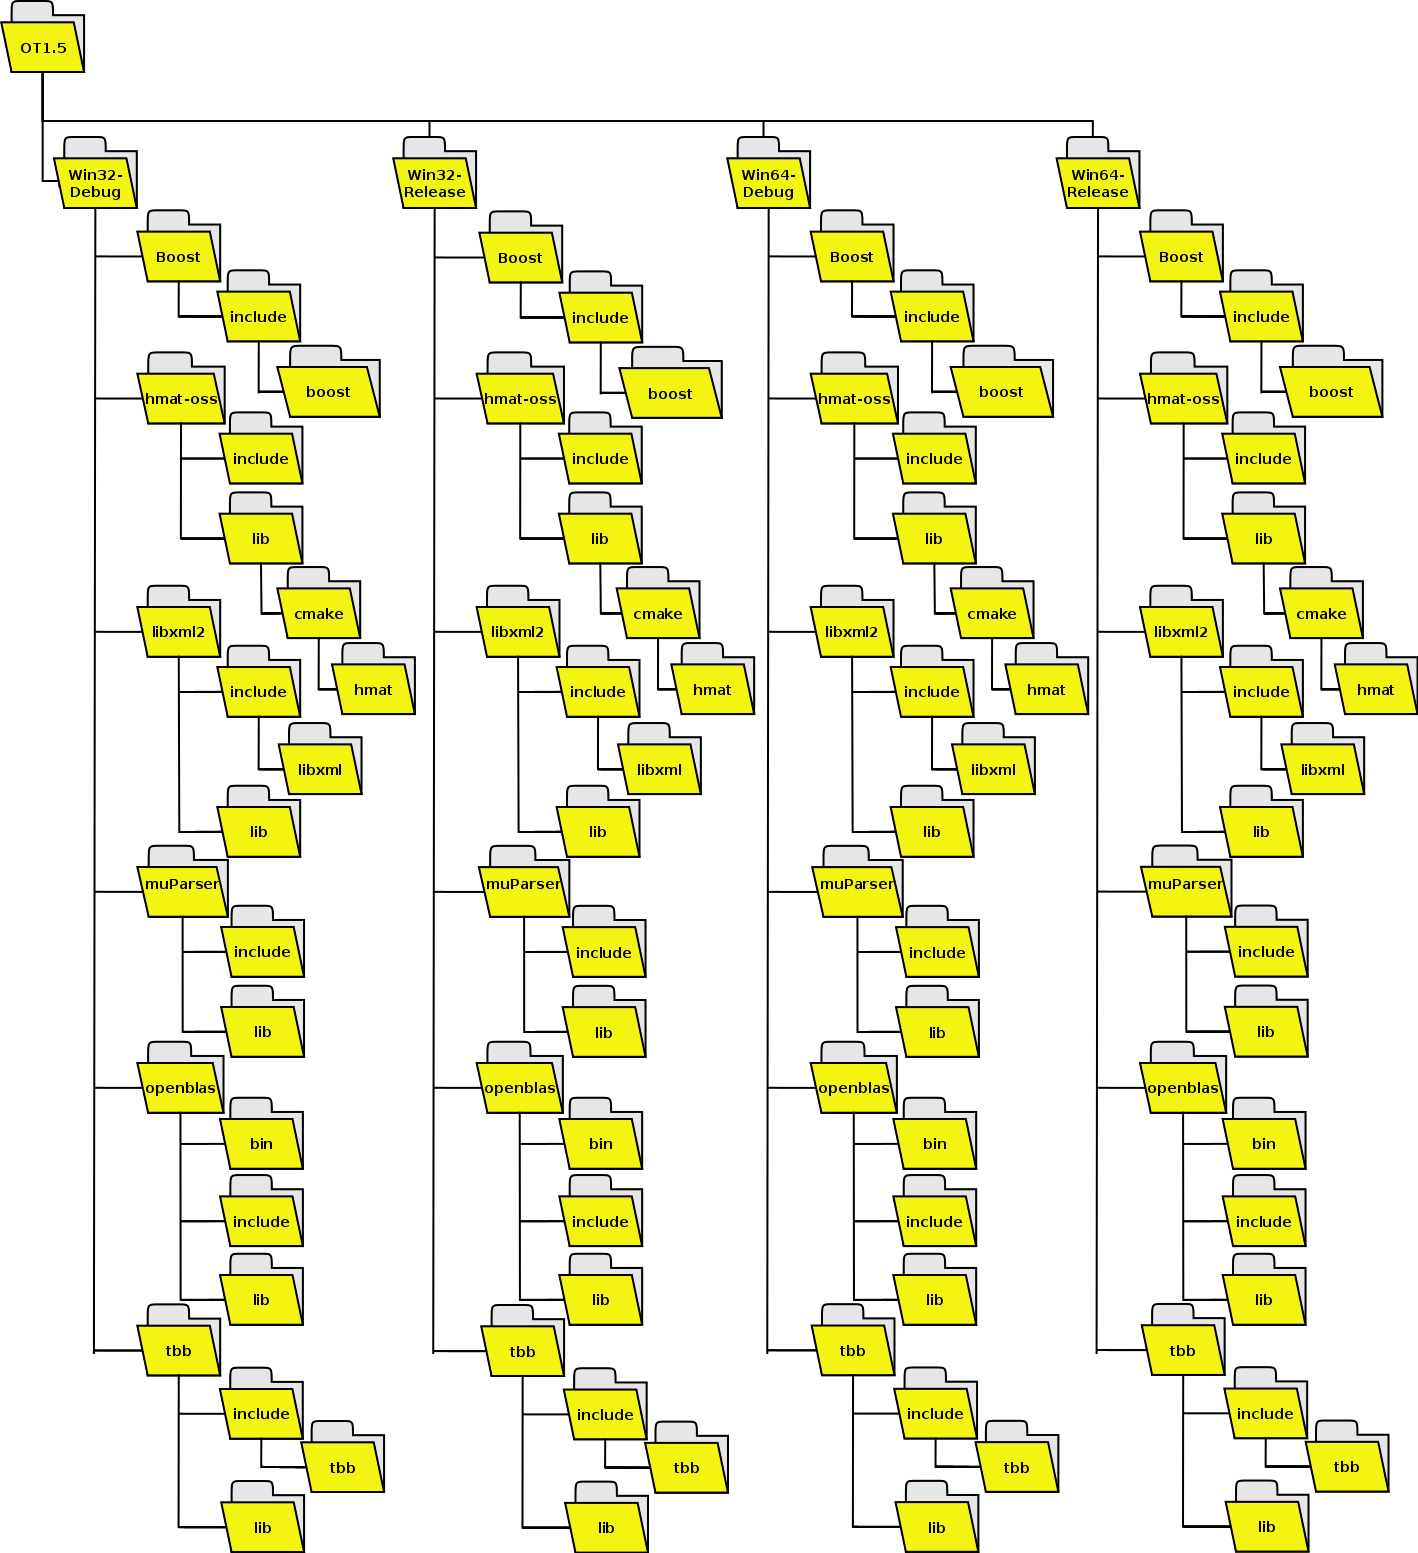
\includegraphics[scale=0.33]{Figures/win_native/win-inst-layout.png}
\caption{Windows installation layout}\label{fig:win-inst-layout}
\end{center}
\end{figure}

For convenience, all libraries will be compiled as static libraries, except OpenBLAS.

\subsubsection{Build and install OpenBLAS and TBB}

For different reasons, OpenBLAS and TBB cannot be compiled along with other dependencies.  As explained on
their site, OpenBLAS is currently only supported on Windows with Mingw compiler.  But binaries can be
used with Visual Studio, this is what we will do.  Thus go to
\url{http://sourceforge.net/projects/openblas/files/} and download Windows binaries, for instance
\url{OpenBLAS-v0.2.13-Win32.zip} for Windows 32 bits, and \url{OpenBLAS-v0.2.13-Win64-int32.zip}

Unzip these archives, and copy files to our installation folder:
\begin{itemize}
\item \verb+OpenBLAS-x.y-Win32\bin\libopenblas.dll+ into \verb+Win32-Release\openblas\bin\+ and\\
      \verb+Win32-Debug\openblas\bin\+
\item \verb+OpenBLAS-x.y-Win32\lib\libopenblas.dll.a+ into \verb+Win32-Release\openblas\lib\+ and\\
      \verb+Win32-Debug\openblas\lib\+
\item \verb+OpenBLAS-x.y-Win32\include+ into \verb+Win32-Release\openblas\+ and\\
      \verb+Win32-Debug\openblas\+
\item \verb+OpenBLAS-x.y-Win64-int32\bin\libopenblas.dll+ into \verb+Win64-Release\openblas\bin\+ and\\
      \verb+Win64-Debug\openblas\bin\+
\item \verb+OpenBLAS-x.y-Win64-int32\lib\libopenblas.dll.a+ into \verb+Win64-Release\openblas\lib\+ and\\
      \verb+Win64-Debug\openblas\lib\+
\item \verb+OpenBLAS-x.y-Win64-int32\include+ into \verb+Win64-Release\openblas\+ and\\
      \verb+Win64-Debug\openblas\+
\end{itemize}

Note that DLLs have been compiled with Mingw, and require some Mingw runtime libraries.  They can be found in
\url{http://sourceforge.net/projects/openblas/files/v0.2.12/mingw32_dll.zip} and
\url{http://sourceforge.net/projects/openblas/files/v0.2.12/mingw64_dll.zip}.
They are:
\begin{itemize}
\item \verb+libgcc_s_sjlj-1.dll+, \verb+libgfortran-3.dll+ and \verb+libquadmath-0.dll+ for Win32
\item \verb+libgcc_s_seh-1.dll+, \verb+libgfortran-3.dll+ and \verb+libquadmath-0.dll+ for Win64
\end{itemize}

TBB comes with its own Visual Studio 2010 configuration file, but we did not find how to integrate it into the build system described
below.  Thus the easiest solution is to:
\begin{enumerate}
\item Download TBB sources from \url{https://www.threadingbuildingblocks.org/download}
\item Unpack it.
\item Launch \verb+build\vs2010\makefile.sln+
\item Select \texttt{Win32} or \texttt{x64} architecture, and \texttt{Release} or \texttt{Debug} configuration (not \texttt{Release-MT} or \texttt{Debug-MT}, unless you know what you are doing).
\item If you want to build a static library, edit Properties, tab Configuration Properties, General, Configuration Type, as shown in figure~\ref{fig:vs-tbb-static}
\item Build project.
\item Copy resulting libraries into installation folder:
  \begin{itemize}
  \item \verb+build\vs2010\ia32\Debug\tbb_debug.lib+ into \verb+Win32-Debug\tbb\lib\+
  \item \verb+build\vs2010\ia32\Release\tbb.lib+ into \verb+Win32-Release\tbb\lib\+
  \item \verb+build\vs2010\intel64\Debug\tbb_debug.lib+ into \verb+Win64-Debug\tbb\lib\+
  \item \verb+build\vs2010\intel64\Release\tbb.lib+ into \verb+Win64-Release\tbb\lib\+
  \end{itemize}
\item Copy \verb+include\tbb+ folder into installation folders:
\verb+Win32-Debug\tbb\include+,\\
\verb+Win32-Release\tbb\include+,
\verb+Win64-Debug\tbb\include+
and \verb+Win64-Release\tbb\include+.
\end{enumerate}

\begin{figure}[htb]
\begin{center}
  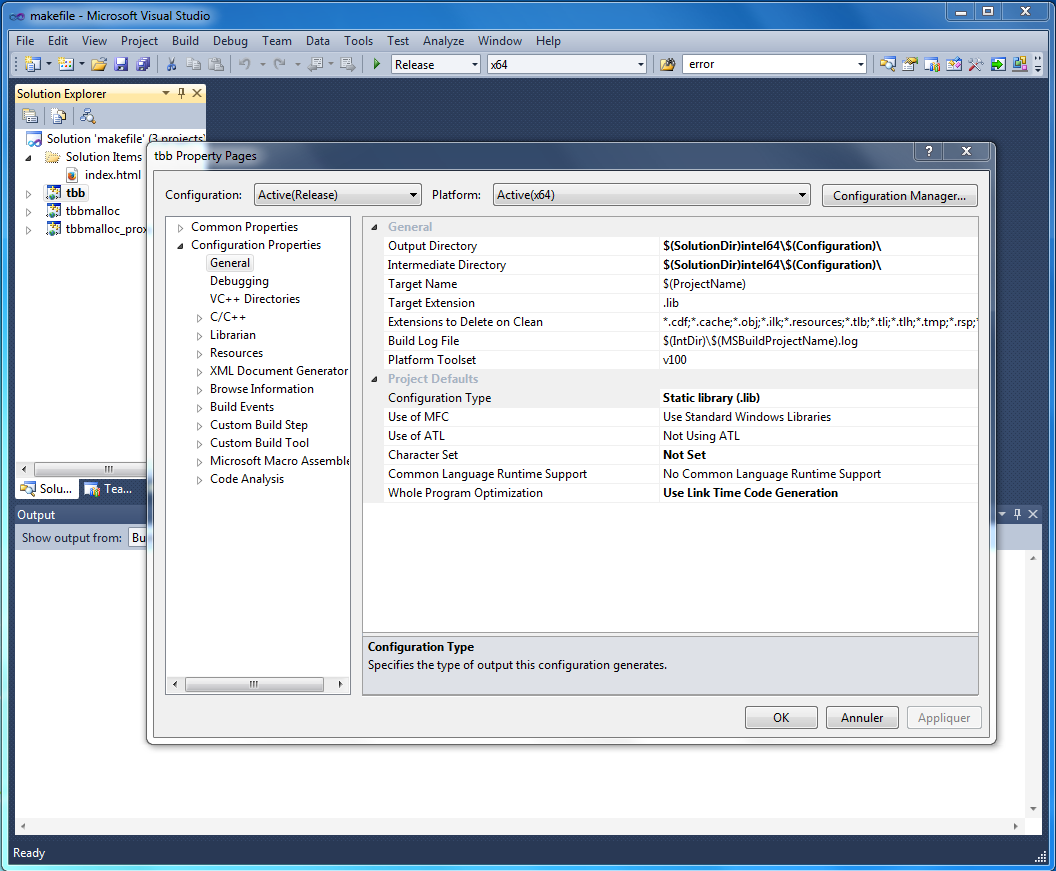
\includegraphics[scale=0.5]{Figures/win_native/vs-tbb-static.png}
\end{center}
\caption{Visual Studio settings to build tbb as a static library}
\label{fig:vs-tbb-static}
\end{figure}

\subsubsection{Build and install OpenTURNS}

OpenBLAS and TBB are low level libraries. Other libraries use STL, and care must be taken to avoid mismatch between runtime
libraries.  To this end, we decided to use a so called \emph{SuperBuild} approach with CMake.  We defined a metaproject
which drives compilation of those dependencies, and also of OpenTURNS itself.
Clone git repository \url{https://bitbucket.org/dbarbier/ot-superbuild} (or download an archive from this URL), launch
\texttt{cmake-gui} program, and follow the following steps:
\begin{enumerate}

\item Launch \texttt{cmake-gui}, and select source and build directories
\begin{center}
  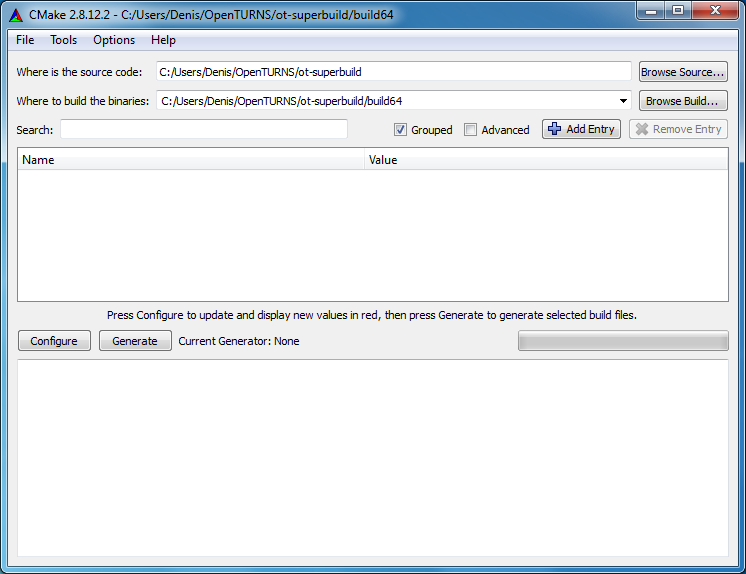
\includegraphics[scale=0.5]{Figures/win_native/cmake-gui-start.png}
\end{center}

\item Click on \textsf{Configure} button.  Select a generator (either Visual Studio 10 or Visual Studio 10 Win64) and compiler
\begin{center}
  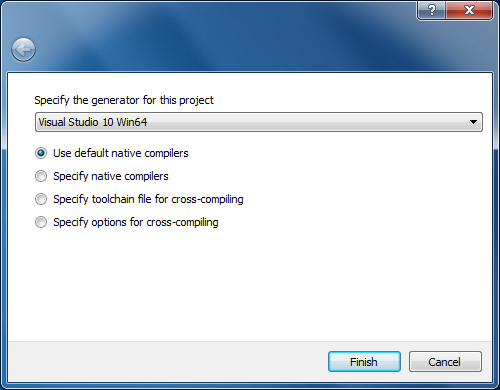
\includegraphics[scale=0.5]{Figures/win_native/cmake-gui-compiler.png}
\end{center}

\item For Win64, CMake may give an error about missing 64-bit tools, as in snapshot below.
Visual Studio Express Edition does not embed 64-bit compilers, and CMake thus checks whether
we are using Express Edition or not.
\begin{center}
  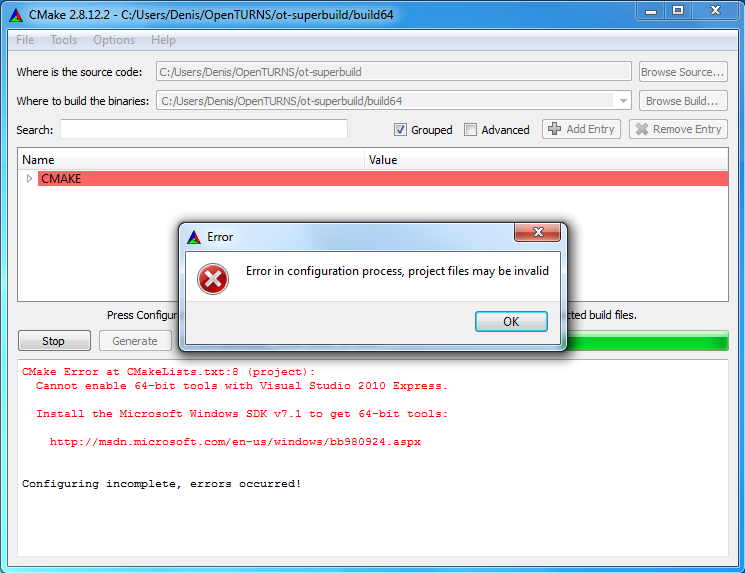
\includegraphics[scale=0.5]{Figures/win_native/cmake-gui-error.png}
\end{center}

It seems that this detection is sometimes buggy; if you know that 64-bit compilers are available,
you can workaround this automatic detection by clicking on \textsf{Add Entry} button, adding a
\texttt{CMAKE\_GENERATOR\_TOOLSET} variable, of type \texttt{STRING}, and value \texttt{v100}.
\begin{center}
  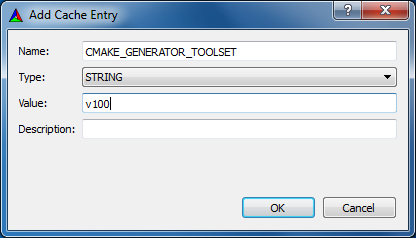
\includegraphics[scale=0.5]{Figures/win_native/cmake-gui-toolset.png}
\end{center}

\item Click on \textsf{Configure} button again, everything should work fine now, and output window should
display \texttt{Configuring done}.

\item Now that CMake has checked that our compiler is working fine, we can tell it where to find OpenBLAS and TBB.
Set \texttt{OPENBLAS\_INCLUDE\_DIR}, \texttt{OPENBLAS\_LIBRARY}, \texttt{TBB\_INCLUDE\_DIR} and
\texttt{TBB\_LIBRARY} variables, as shown below:
\begin{center}
  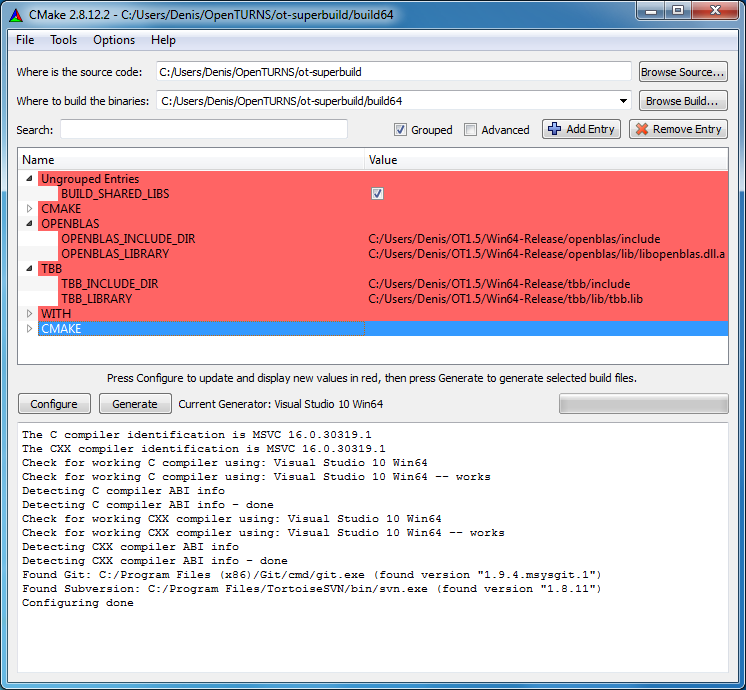
\includegraphics[scale=0.5]{Figures/win_native/cmake-gui-superbuild.png}
\end{center}
and click on \textsf{Configure} button.

\item If everything went fine, click on \textsf{Generate} button.  This generates Visual Studio solution files in the specified
build directory, and you can now close \texttt{cmake-gui} window.

\item Launch \texttt{openturns-superbuild} solution file.
\begin{center}
  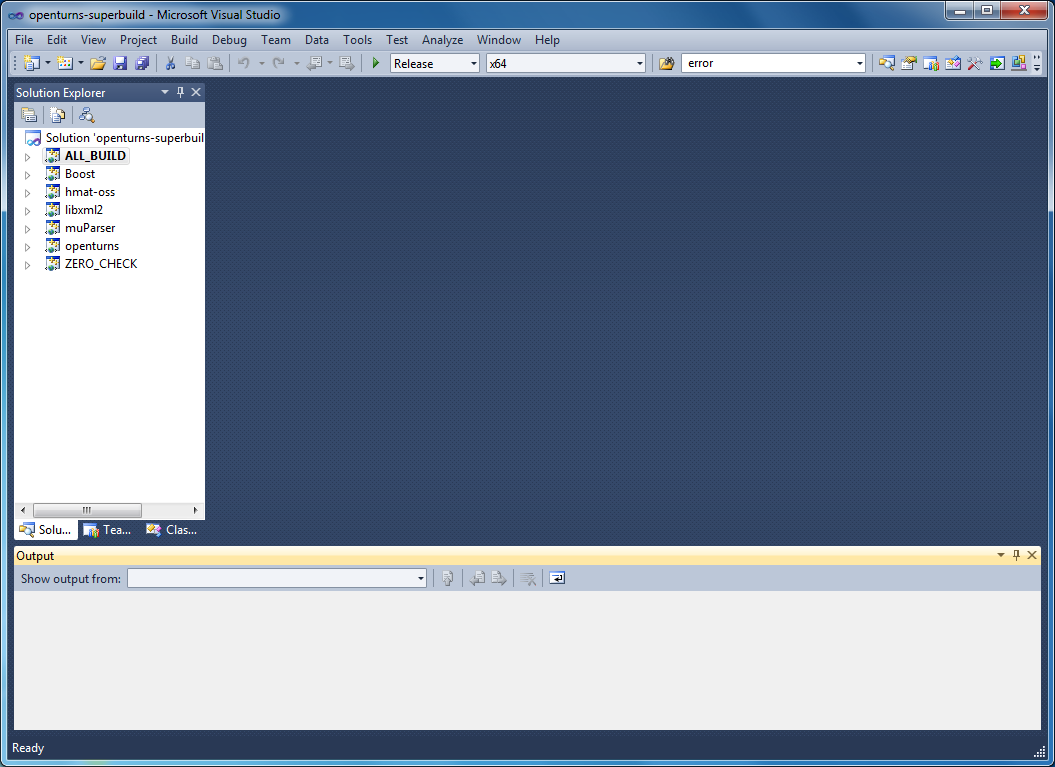
\includegraphics[scale=0.5]{Figures/win_native/vs-superbuild.png}
\end{center}
Select \texttt{Release} or \texttt{Debug} configuration (it must match TBB configuration), and build solution file.
This will download sources (a working Internet connection is thus required), unpack and build them.
It can take a long time on a slow machine, or with a slow Internet connection, since some downloaded sources are large.
\item Copy \verb+build64\ExternalProjects\Install\*+ directories into installation prefix (\verb+OT1.5\Win64-Release\+, or \verb+Win32-Release+,
etc)
\end{enumerate}

\subsection{Manual compilation}

If you want to modify settings, the simplest solution is to proceed as in previous section, and modify Visual Studio settings afterwards.
Dependencies are downloaded, built and installed into an \verb+ExternalProjects+ subdirectory of build directory, ie
\verb+build64\ExternalProjects+ in our example.  This directory contains the following folders:
\begin{itemize}
\item \texttt{Build}: contains generated Visual Studio projects, and files generated during builds
\item \texttt{Download}: contains project archives
\item \texttt{Install}: after build, each project installs resulting files (header files and libraries) there
\item \texttt{Source}: unpacked source files
\item \texttt{Stamp}: keeps track of already processed steps
\item \texttt{tmp}
\end{itemize}
Each directory in turn contains one directory per project.  Thus if one wants to modify some settings when compiling OpenTURNS,
one has to go to \verb+build64\ExternalProjects\Build\openturns\+ directory and launch the Visual Studio solution file found there,
in this case \texttt{OpenTURNS.sln}.  For instance, one can build OpenTURNS tests from this solution file.
Beware to always check that active configuration is the desired one.

\subsection{Unresolved problems}
\paragraph{Python bindings are not generated}

After installing SWIG and Python binaries, we had been able to generate Python modules without trouble, but Python could not load
those modules.  It seems that the same version of Visual Studio must be used to compile Python and modules, but we could only find
Python binaries built with Visual Studio 9.  The solution is to build Python from sources, but this had not been tested yet.

\paragraph{Tests are not run}

Tests can be compiled but not launched from Visual Studio, because they are run via shell commands, and also because tests executable are
generated in a subdirectory.  It is possible to work around those limitations and run tests, but this is currently not automated.

\subsection{Troubleshooting}
\begin{itemize}
\item It is possible to build multiple configurations with Visual Studio solution files, but this is currently not supported by
our \texttt{CMakeLists.txt} files; thus one must launch \texttt{cmake-gui}, adapt variables (for instance paths to OpenBLAS
and TBB libraries must be modified for each configuration) and press \textsf{Configure} and \textsf{Generate} buttons.
\item No OpenBLAS library in \texttt{Debug} mode is provided, but the one from \texttt{Release} mode works also in \texttt{Debug}
mode.  On the other hand, OpenTURNS and TBB configurations must match, it is not possible to link OpenTURNS in \texttt{Debug} mode
against TBB in \texttt{Release} mode, or vice-versa.
\item Boost contains files with very long filenames, which causes trouble on NTFS.  If you have already built Boost and want to
build it again, Visual Studio may complain that it encountered an error when building it again.  In that case, launch file
explorer and remove Boost directory, then press again \textsf{Generate} button of CMake (because some of its generated files had
been removed too), it should now build fine.
\end{itemize}

\cleardoublepage

\ifpdf
\cleardoublepage
\phantomsection
\addcontentsline{toc}{section}{Index}
\fi
\printindex
\end{document}
